\documentclass{article}
\usepackage{graphicx}
\DeclareGraphicsExtensions{.pdf}

\usepackage[final]{pdfpages}

\headheight 0in
\oddsidemargin 0in
\evensidemargin  0in
\topmargin  -.25in
\textwidth 6.5in
\textheight 9in
\title{OMPT: An OpenMP\textsuperscript{\textregistered} Tools Application Programming Interface for Performance Analysis}
\author{Alexandre Eichenberger\thanks{IBM T.J. Watson Research Center}, 
John Mellor-Crummey\thanks{Rice University}, 
Martin Schulz\thanks{Lawrence Livermore National Laboratory},
\\~\\
Nawal Copty\thanks{Oracle}, 
Jim Cownie\thanks{Intel},
% John DelSignore\thanks{Rogue Wave}, 
Robert Dietrich\thanks{TU Dresden, ZIH},
Xu Liu\hbox to 0in{$^\dagger$\hss},
Eugene Loh\hbox to 0in{$^\S$\hss}, 
Daniel Lorenz\thanks{J\"{u}lich Supercomputer Center}, 
\\
and other members of the OpenMP Tools Working Group}
\date{March 21, 2014}

\usepackage{comment}
\usepackage{needspace}
\usepackage[colorlinks=true,citecolor=blue]{hyper ref}
\usepackage{url}
\usepackage{xcolor}

\newcommand{\descheader}[1]{{\needspace{3\baselineskip}\vspace{1em}\noindent \fbox{#1}}}


\begin{document}     
\pagestyle{empty}
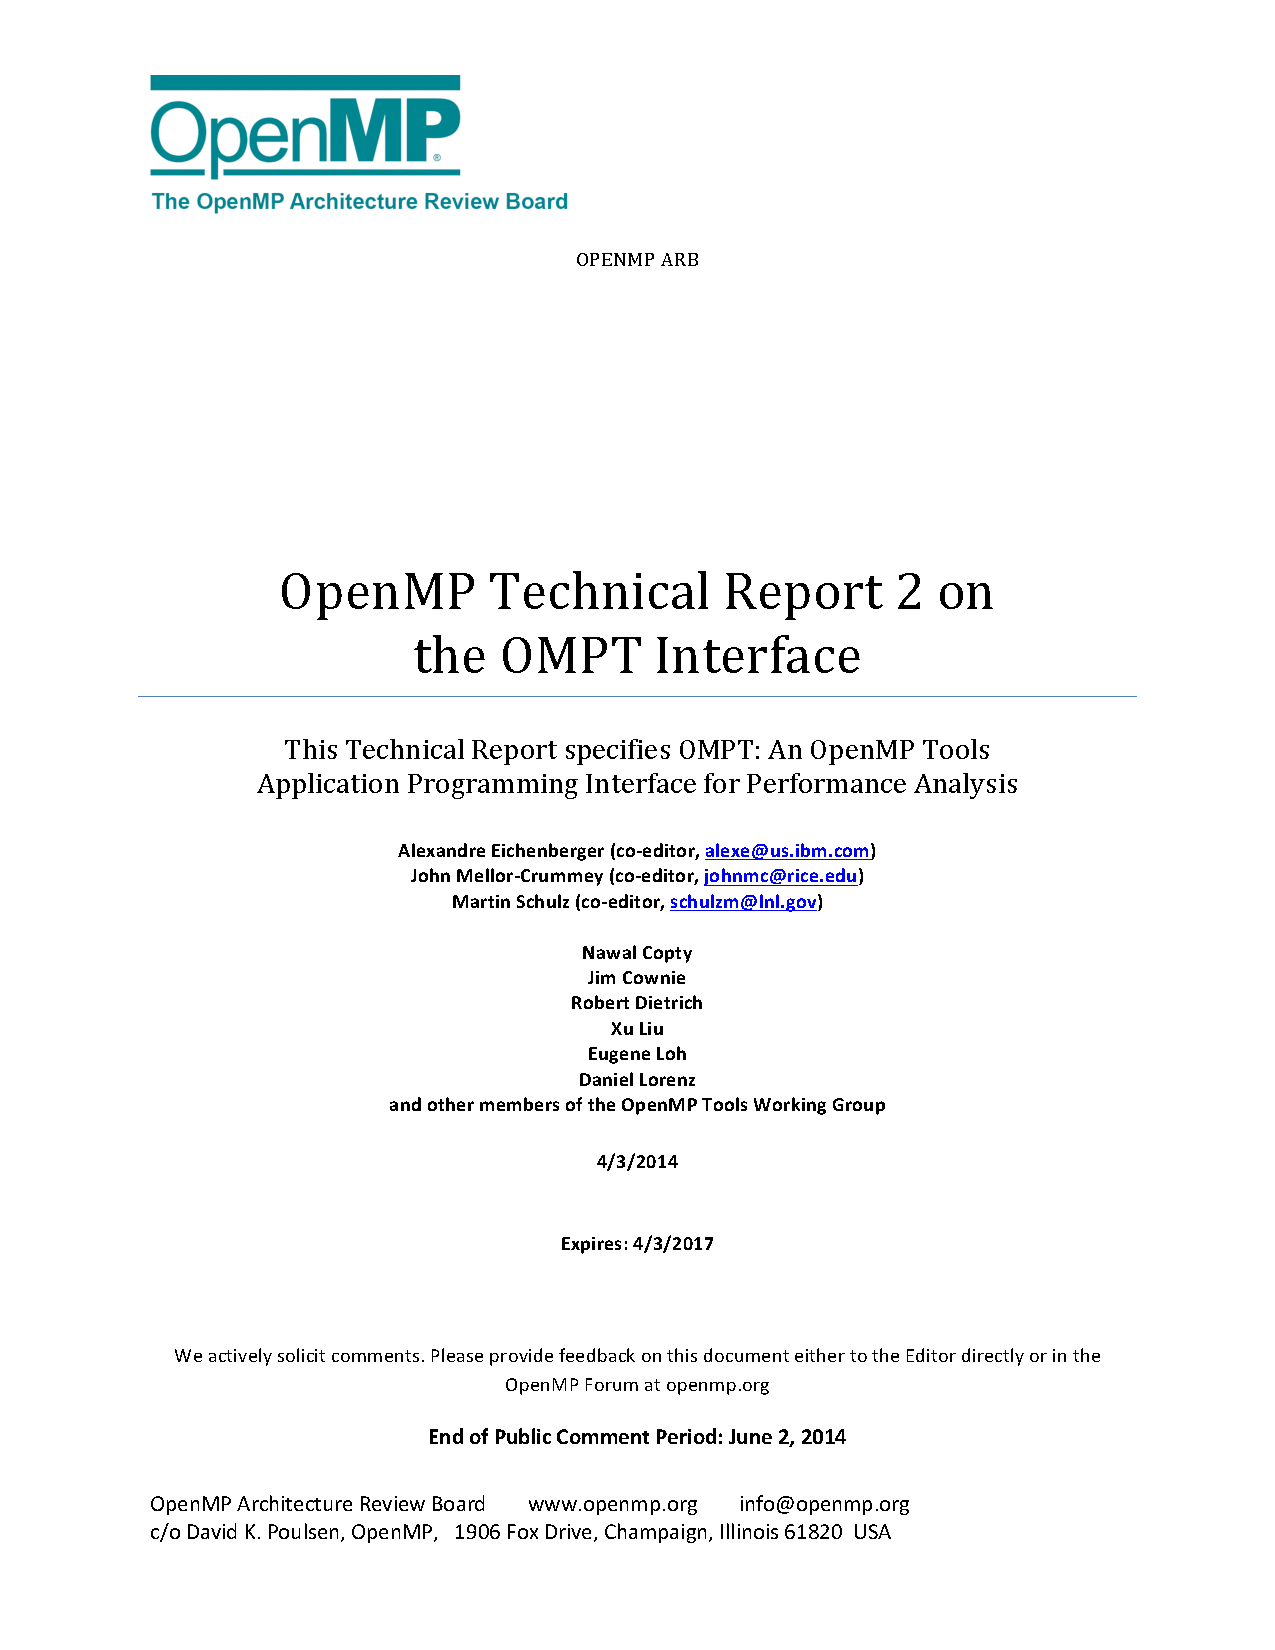
\includepdf[
   pages={-},
   pagecommand={},
 ]{OMPT_TR_header}
 
\setcounter{page}{1}
\pagestyle{plain}
                                           
\maketitle
\section{Introduction}
Today, it is difficult to produce high quality tools that support 
% debugging and/or 
performance analysis of OpenMP programs without tightly integrating them with a specific OpenMP runtime implementation. To address this problem, this document defines OMPT---an application programming interface (API) for first-party performance tools.\footnote{A {\em first-party} tool runs within the address space of an application process. This differs from a {\em third-party} tool, e.g., a debugger, which runs as a separate process.}  
Extending the OpenMP standard with this API  will make it possible to construct powerful tools that will support any standard-compliant OpenMP implementation.


\begin{comment}
In appendices, we
define OMPD---an optional shared-library plugin that will enable debuggers  to inspect and control executions of OpenMP programs. We describe OMPD in this document because it provides third-party variants  of OMPT features  to enable assembly of user-level views of thread call stacks by debuggers.
\end{comment}

\subsection{OMPT}

The design of OMPT is based on experience with two prior efforts to define a standard OpenMP tools API: the POMP API~\cite{Mohr:EWOMP02} and the Sun/Oracle Collector API~\cite{SunCollector,Jost:2005:AND:1892830.1892858}. 
The POMP API provides support for instrumentation-based measurement. A drawback of this approach  is that its overhead can be significant because an operation, e.g., an iteration of an OpenMP worksharing loop, may take less time than tool callbacks monitoring its execution. 
%Doesn't have to be:
%Second, traces grow quickly and can be unwieldy for long executions. 
In contrast, 
the Sun/Oracle Collector API was  designed primarily to support performance measurement 
% and attribution of performance information 
using asynchronous sampling. This  design enables the construction of tools that attribute costs without the overhead and intrusion of pervasive instrumentation. With the Collector API, tools
 can use low-overhead asynchronous  sampling of application call stacks to record compact call path profiles. However, the Collector API doesn't provide enough instrumentation hooks to provide full tool support for statically-linked executables.
% instrumentation hooks to enable construction of trace analyzers or verification tools.
OMPT builds upon ideas from both the POMP and  Collector APIs. The core of OMPT is a minimal set of features to support tools that employ asynchronous sampling to measure application performance. In addition, OMPT defines  interfaces to support  {\em blame shifting}~\cite{Tallent:PPoPP09,Tallent:PPoPP10}---a technique that shifts attribution of costs from symptoms to causes.
Finally, OMPT defines callbacks suitable for instrumentation-based monitoring of runtime events. 
 OMPT can be implemented entirely by a compiler, entirely by an OpenMP runtime system, or with a hybrid strategy that employs a mixture of compiler and runtime support.
%equires no compiler support, and is implemented entirely within an OpenMP runtime system. 

With the exception of one routine for tool control, all functions in the OMPT API are intended for use only by tools rather than by applications. All OMPT API functions  have a C binding. A Fortran binding is  provided only for the single application-facing tool control function described in Section~\ref{sec:app-facing}.

\subsubsection{Design Objectives}
OMPT tries to satisfy several design objectives for a performance tool interface for OpenMP. These objectives are listed in decreasing order of importance.
\begin{itemize}
\item The  API should enable tools to gather sufficient information about an OpenMP program execution  to associate costs with both the program and the OpenMP runtime system.
\begin{itemize}
\item The  API should provide an interface sufficient to construct low-overhead performance tools based on asynchronous sampling.
\item The API should enable a profiler that uses call stack unwinding to identify which frames in its call stack are present on behalf of the OpenMP runtime.
\item An OpenMP runtime system should associate the activity of a thread at any point in time with a {\em state}, e.g., idle, which will enable a performance tool to interpret program behavior.  
\item Certain API routines must be defined as {\em async signal safe} so that they can be invoked in a profiler's signal handler as it processes interrupts generated by asynchronous sampling.
\end{itemize}
\item Incorporating support for the  API in an OpenMP runtime system should add negligible overhead to the runtime system if the interface is not in use by a tool.
\item The API should define interfaces suitable for constructing  instrumentation-based performance tools.
\item Adding the API to an OpenMP runtime should not impose an unreasonable development burden on the runtime developer.
\item The API should not impose an unreasonable development burden on tool implementers.
\end{itemize}

To support the OMPT interface for tools, an OpenMP runtime system must maintain information about the state of each OpenMP thread and provide a set of API calls that tools can use to interrogate the OpenMP runtime. Maintaining information about the state of each thread in the runtime system is not free and thus an OpenMP runtime system need not maintain state information unless a tool has registered its interest in this information.
% , or an environment variable has directed the tool to track runtime state.
Without any explicit request to enable tool support, an OpenMP runtime need not maintain any state for the benefit of tools.

\subsubsection{Minimally Compliant Implementation}

OMPT has a small set of mandatory features that provide a common foundation for all performance tools. A runtime may also implement additional, optional, OMPT features used by some tools to gather extra information about a program execution.     
The features required by a minimally compliant implementation are summarized below.

\begin{itemize}
\item Maintain a unique numerical ID per OpenMP thread, parallel region, and task region. A minimal implementation may reuse the task ID required by OpenMP for nested locks.
\item Maintain pointers into the stack for each OpenMP thread to distinguish frames for user procedures from frames for OpenMP runtime routines.  Each  OpenMP worker must maintain a pointer to the stack frame of the runtime routine containing its idle loop, if one exists on the stack. 
\item Maintain a state and a wait condition for each OpenMP thread. Mandatory states are idle, work serial, work parallel, and undefined.
\item Provide callbacks to tools when encountering the following  events:  thread begin/end, parallel region begin/end, task region begin/end, a user-level tool control call, and runtime shutdown.
\item Implement several async signal safe inquiry functions to retrieve information from the OpenMP runtime.
\item Have the OpenMP runtime initiate a callback to a tool initialization routine 
as directed by the value of a new OpenMP environment variable (\verb|OMP_TOOL|) and provide a function to register tool callbacks with the runtime.
\end{itemize}

\subsection{Document Roadmap}
This document first outlines various aspects of the OMPT tools API. 
Section~\ref{sec:states} describes the state information maintained by the OpenMP runtime system on behalf of OMPT for use by tools.
Section~\ref{sec:events} describes the OMPT callbacks to notify a tool of various OpenMP runtime events during an execution.
Section~\ref{sec:data} describes the data structures used by the OMPT interface.
Section~\ref{sec:inquiry} describes the runtime system inquiry operations supported by OMPT for the benefit of tools.
Section~\ref{sec:enabling} describes the OMPT API operations for tool initialization.
% Section~\ref{sec:globals} describes a global variable provided by the OpenMP runtime to support the OMPD debugger plug in library, which is being developed separately.
Section~\ref{sec:app-facing} describes the tool control interface available to applications.
Section~\ref{sec:notes} concludes with a few notes about potential future enhancements.
Appendix~\ref{appendix:ompt-types} provides a definition of the complete OMPT interface in C.
Appendix~\ref{app:frame} illustrates the information that OMPT maintains about call stacks and the use of OMPT API routines to inspect it; this support enables tools to associate code executed in OpenMP parallel regions with  application-level calling contexts. 

\begin{comment}
Next, a pair of appendices describe OMPD---a shared library plugin for debuggers that supports third-party inspection and control of a target process. OMPD enables a debugger to leverage functionality provided by OMPT to enable it to provide a user-level view of call stacks for threads.
Appendix~\ref{appendix:ompd} describes the OMPD interface.  
Appendix~\ref{appendix:ompd-types} provides a definition of the complete OMPD interface in C.
\end{comment}

\section{Runtime States} 
\label{sec:states} 

To enable a tool to understand what an OpenMP thread is doing, when a tool registers itself with an OpenMP runtime system, the runtime 
will maintain state information for each OpenMP thread that can be queried by the tool. 
The state maintained for each thread by the OpenMP runtime is an
approximation of the thread's instantaneous state. 
OMPT uses the enumeration type \verb|ompt_state_t| for states;
Appendix~\ref{appendix:ompt-types:states} defines this type.
When the state of a thread not associated with the OpenMP runtime is queried, the runtime returns 
\verb|ompt_state_undefined|.

For each OpenMP thread the runtime maintains not only a state but also an \verb|ompt_wait_id_t|
identifier.  When a thread is waiting for a lock, critical region,
ordered, or atomic, and the thread is in a wait
state, then 
the thread's \verb|wait_id| field identifies the lock, critical construct, ordered construct, atomic construct, or internal variable
upon which the
thread is waiting. The semantics of the values used for a \verb|wait_id| are implementation defined.
A thread's \verb|wait_id| is undefined if the thread
is not in a wait state.

States are classified as {\em mandatory}, {\em optional}, or {\em flexible}. 
Flexible states provide an OpenMP runtime with leeway to determine if
and when to report transitions to a flexible state.
For example, consider when a thread acquires a lock. One
compliant runtime may transition a thread's state to 
\verb|ompt_state_wait_lock| (flexible state) early before the thread attempts to acquire a
lock. Another compliant runtime may transition a thread's state to
\verb|ompt_state_wait_lock| late, only if the thread begins to spin or
block to wait for an unavailable lock. A third compliant runtime
may transition a thread's state to \verb|ompt_state_wait_lock| even later, e.g., only
after the thread waits for a significant amount of time. 
% While flexible states are not mandatory as ``significant amount of time" is  not precisely defined, implementing them is recommended.

State values 0 to 127 are reserved for current OMPT states and future extensions.  

\descheader{Idle State}

\begin{description}
\item \verb|ompt_state_idle| (mandatory)

  The thread is idle while waiting to work on an OpenMP parallel
  region.
\end{description}

\descheader{Work States}

\begin{description}

\item \verb|ompt_state_work_serial| (mandatory)

  The thread is executing code outside all parallel regions. 

\item \verb|ompt_state_work_parallel| (mandatory)

  The thread is executing code within the scope of a parallel region construct.

\sloppy
\item \verb|ompt_state_work_reduction| (optional)
 
  The thread is combining partial reduction results from threads in its team. A compliant
  runtime might never report a thread in this state; a thread
  combining partial reduction results may  report its state as
  \verb|ompt_state_work_parallel| or \verb|ompt_state_overhead|.

\end{description}

\descheader{Barrier Wait States}

\begin{description}

  \item \verb|ompt_state_wait_barrier| (flexible)
  
  \sloppy
  The thread is waiting at either an implicit or explicit barrier.
  A  compliant implementation may have a thread enter this state
  early, when the thread encounters a barrier, or late, when the
  thread begins to wait at the barrier. A  compliant implementation may never report a thread in this state; instead a thread might report its state as \verb|ompt_state_wait_barrier_implicit|  or \verb|ompt_state_wait_barrier_explicit|, as appropriate.
  
  \item \verb|ompt_state_wait_barrier_implicit| (flexible)
  
\sloppy
  The thread is waiting at an implicit barrier in a parallel region. 
  A  compliant implementation may have a thread enter this state
  early, when the thread encounters a barrier, or late, when the
  thread begins to wait at the barrier.
  A  compliant runtime implementation may report \verb|ompt_state_wait_barrier| for implicit barriers.
  
    \item \verb|ompt_state_wait_barrier_explicit| (flexible)

  The thread is waiting at an explicit barrier  in a parallel region. 
  A  compliant implementation may have a thread enter this state
  early, when the thread encounters a barrier, or late, when the
  thread begins to wait at the barrier.
  A  compliant runtime implementation may report \verb|ompt_state_wait_barrier| for explicit barriers.
  
\end{description}
  
\descheader{Target Wait States}

\begin{description}

\item \verb|ompt_state_wait_target| (flexible)

  The thread is waiting at a target construct. A compliant
  implementation may have a thread enter this state early, when the
  thread encounters a target construct, or late, when the thread
  begins to wait for the target region to complete.
  
\item \verb|ompt_state_wait_target_data_map| (optional)

  The thread is waiting for a target data map operation to complete.

\end{description}
  
\descheader{Task Wait States}

\begin{description}

\item \verb|ompt_state_wait_taskwait| (flexible)

  The thread is waiting at a taskwait construct. A compliant
  implementation may have a thread enter this state early, when the
  thread encounters a taskwait construct, or late, when the thread
  begins to wait for an uncompleted task.

\item \verb|ompt_state_wait_taskgroup| (flexible)

  The thread is waiting at the end of a taskgroup construct. A compliant
  implementation may have a thread enter this state early, when the
  thread encounters the end of a taskgroup construct, or late, when the thread
  begins to wait for an uncompleted task.

\end{description}


\descheader{Mutex Wait States}

\begin{description}

\item \verb|ompt_state_wait_lock| (\verb|ompt_state_wait_nest_lock|) (flexible)

  The thread is waiting for a  lock (nest lock). A compliant implementation
  may have a thread enter this state early, when a thread
  encounters a lock (nest lock) \verb|set| routine, or late, when the thread
  begins to wait for a lock (nest lock).

  Before a thread enters this state, the OpenMP runtime system will
  update the thread's \verb|ompt_wait_id_t| field to identify the lock (nest lock) being acquired.

\item \verb|ompt_state_wait_critical| (flexible)

  The thread is waiting to enter a critical region. A compliant
  implementation may have a thread enter this state early, when the
  thread encounters a critical construct, or late, when the thread
  begins to wait to enter the critical region. A compliant
  implementation may report a thread waiting to enter a critical
  region in \verb|ompt_state_wait_lock| if waiting for a lock associated with the construct.

  Before a thread enters this state, the OpenMP runtime system will
  update the thread's \verb|ompt_wait_id_t| field to identify the critical construct or an internal runtime variable (e.g., a lock) associated with the critical construct.

\item \verb|ompt_state_wait_atomic| (flexible)

  The thread is waiting to enter an atomic region. A compliant
  implementation may have a thread enter this state early, when the thread
  encounters an atomic construct, or late, when the thread begins
  to wait to enter the atomic region. A compliant
  implementation may report a thread waiting to enter an atomic
  region in \verb|ompt_state_wait_lock| if waiting for a lock associated with the atomic construct.
  A compliant implementation may opt to not report
  this state, for example, when using atomic hardware instructions, which allow non-blocking atomic implementations.

  Before a thread enters this state, the OpenMP runtime system will
  update the thread's \verb|ompt_wait_id_t| field to identify the atomic construct, a program variable, or an internal runtime variable (e.g., a lock) associated with the atomic construct.


\item \verb|ompt_state_wait_ordered| (flexible)

  The thread is waiting to enter an ordered region. A compliant
  implementation may have a thread enter this state early, when the thread encounters
  an ordered construct, or late, when the thread begins
  to wait to enter the ordered region. A compliant
  implementation may report a thread waiting to enter a ordered
  region in \verb|ompt_state_wait_lock| if waiting for a lock associated with the ordered construct.

  Before a thread enters this state, the OpenMP runtime system will
  update the thread's \verb|ompt_wait_id_t| field to identify the ordered construct or an internal runtime variable (e.g., a lock) associated with the ordered construct.
  
  \end{description}

\descheader{Overhead State}

\begin{description}

\item \verb|ompt_state_overhead| (optional)

  A thread may be reported as being in the overhead state at any point while executing within an OpenMP runtime system, e.g., while
    preparing a parallel region, 
    preparing a new explicit task,
    preparing a worksharing region, or
    preparing to execute iterations of a parallel loop.  
  It is compliant to report some or all OpenMP runtime overhead 
  as work.

\end{description}

\descheader{Miscellaneous States}

\begin{description}

\item \verb|ompt_state_undefined| (mandatory)

  This state is reserved for threads that are not user threads,
  initial threads, threads currently in an OpenMP team, or threads
  waiting to become part of an OpenMP team.


\item \verb|ompt_state_first| (mandatory)

\sloppy
  This state is a placeholder exclusively reserved for use by the OMPT runtime call \verb|ompt_enumerate_state| (see Section~\ref{ompt_enumerate_state}), which is used to enumerate all available runtime states. A thread will never be reported in this state.

\end{description}

\section{Events}
\label{sec:events} 

This section describes callback events that an OpenMP runtime 
may provide for use by a tool. OMPT uses the enumeration type \verb|ompt_event_t| for events; 
Appendix~\ref{appendix:ompt-types:events} defines this type. 
A tool need not register a callback for any particular event.
In most cases, an OpenMP runtime system will not make any callback unless a  tool has registered to receive it. The exception to this rule is begin/end event pairs. 
To implement event notifications efficiently, a runtime may assume that for certain begin/end event pairs if one event of the pair has a callback registered, the other will have a callback defined as well. When this exception applies, it will be noted for affected events.

Callbacks for different events may have different type signatures. 
The type signature for an event's callback is noted with the event definition.  Appendix~\ref{appendix:ompt-types:callbacks} defines type signatures for callback events.


There are two classes of events: mandatory events and optional events.
Mandatory events must be implemented in any compliant OpenMP runtime implementation. 
Optional events are grouped in sets of related events. Except for begin/end pairs as noted, support for any particular optional event can be included or omitted at the 
discretion of a runtime system implementer. 


\subsection{Mandatory Events}

 The following callback events are mandatory and must be supported by a compliant OpenMP 
 runtime system. 

\descheader{Threads}

\begin{description}

\begin{comment}
\item \verb|ompt_event_initial_thread_begin|

% def of initial thread: A thread that executes an implicit parallel region.
% def of implicit parallel region: An inactive parallel region that generates an initial task region. Implicit parallel regions surround the whole OpenMP program, all target regions, and all teams regions.

The OpenMP runtime invokes this callback when an initial thread triggers initialization of the OpenMP runtime for itself. 
The runtime issues the callback after the runtime is fully initialized, but before the thread executes any
OpenMP tasks. The callback executes in the context of the initial thread and must precede any other callbacks for that thread.
This callback has type signature \verb|ompt_thread_callback_t|. 
\end{comment}

% def of openmp thread: A thread that is managed by the OpenMP runtime system.

\item \verb|ompt_event_thread_begin|

The OpenMP runtime invokes this callback in the context of an initial thread just after it initializes the OpenMP runtime for itself, or in the context of a new thread created by the OpenMP runtime system just after the thread initializes itself. In either case, this callback must be the first callback for a thread
and must occur before the thread executes any OpenMP tasks. The type of the thread (\verb|ompt_thread_initial|, \verb|ompt_thread_worker|, or \verb|ompt_thread_other|) is passed as an argument to the callback. This callback has type signature \verb|ompt_thread_type_callback_t|. 


\item \verb|ompt_event_thread_end|

The OpenMP runtime invokes this callback
after an OpenMP thread completes all of
its tasks but before the thread is destroyed. The callback
executes in the context of the OpenMP thread. This callback must be the last callback event for any thread of type \verb|ompt_thread_worker|; it is optional for other types of threads.
This callback has type signature \verb|ompt_thread_type_callback_t|. 

\end{description}

\descheader{Parallel Regions}

\begin{description}

\item \verb|ompt_event_parallel_begin|

\sloppy
The OpenMP runtime invokes this callback 
after a task encounters a parallel construct
but before any implicit task starts to execute the
parallel region's work. The callback executes in the context of the task that encountered the parallel construct.
This callback has type signature \verb|ompt_new_parallel_callback_t|, and includes a parameter that indicates the number of threads requested by the user. 
A tool may use this value as an upper bound on the number of threads that will participate in the team.

\item \verb|ompt_event_parallel_end|

The OpenMP runtime invokes this callback 
after a parallel
region executes its closing synchronization barrier but before
resuming execution of the parent task.  The callback executes in
the context of the task that encountered the parallel construct.
This callback has type signature \verb|ompt_parallel_callback_t|. 

\end{description}

\descheader{Target Regions}

\begin{description}

\item \verb|ompt_event_target_begin|

  The OpenMP runtime invokes this callback after a task encounters a target construct but before the region is executed by a device.
  The callback executes in the context of the task that encountered the target construct.
  This callback has type signature \verb|ompt_new_target_callback_t|.

\item \verb|ompt_event_target_end|

  The OpenMP runtime invokes this callback after the region is executed by a device but before the encountering task leaves the target region.
  This callback has type signature \verb|ompt_target_callback_t|.
  
\end{description}

\descheader{Tasks}

\begin{description}

\item \verb|ompt_event_task_begin|
 
The OpenMP runtime invokes this callback
after a task encounters a task construct
but before the new explicit task 
executes. The callback executes in the context of
the task that encountered the task construct.
This callback has type signature \verb|ompt_new_task_callback_t|.

\item \verb|ompt_event_task_end|   
 
\sloppy
The OpenMP runtime invokes this callback
after an explicit task
completes but before the thread resumes execution of another
task.  The callback executes in the context of an
arbitrary task on the thread that completed the explicit task.
This callback has type signature \verb|ompt_task_callback_t|. 

\end{description}


\descheader{Application Tool Control}

\begin{description}

\item \verb|ompt_event_control|

If the user program calls \verb|ompt_control|, the
OpenMP runtime invokes this callback.
The callback executes in the environment
of the user control call; the arguments passed to the callback are the values passed by the user to \verb|ompt_control|.
This callback has type signature \verb|ompt_control_callback_t|. 

\end{description}

\descheader{Termination}

\begin{description}

\item \verb|ompt_event_runtime_shutdown|
 
The OpenMP runtime system invokes this callback before it shuts down the
 runtime system.  This callback enables a tool to clean up its
 state and record or report its measurement data, as appropriate. A runtime may later restart and reinitialize the tool by
calling the tool initializer
function (\verb|ompt_initialize|, described in Section~\ref{sec:init}) again.
 This callback has type signature \verb|ompt_callback_t|. 


\end{description}

\subsection{Optional Events}
This section describes two sets of events. 
The first set of events is intended primarily for use by sampling-based performance tools that 
employ a strategy known as {\em blame shifting} to attribute waiting to activity in
 contexts that cause other threads to wait
rather than contexts in which waiting is observed.
The second set of events, in combination with other mandatory and optional events, 
enables instrumentation-based tools to receive notification for any or all OpenMP runtime events as they occur.
 
Support for these events is optional. An OpenMP runtime system remains compliant even if it supports none of the events in this section.


\subsubsection{Events for Blame Shifting (Optional)}
\label{sec:blame}
This section describes callback events used by sampling-based performance tools 
that employ {\em blame shifting} to transfer blame for waiting from contexts 
where waiting is observed to contexts responsible for the waiting.\footnote{The utility of blame shifting has previously been demonstrated for attributing 
idling while waiting to steal work 
in a work-stealing runtime~\cite{Tallent:PPoPP09}, and spin waiting to acquire a lock~\cite{Tallent:PPoPP10}.}
Using these callbacks, a tool employing blame shifting 
can attribute time that a thread spends waiting for a lock to the context of the lock holder.
Similarly, time that threads spend waiting at a barrier can be attributed back 
to code being executed by working threads while other threads wait.

The events listed immediately below are used by an OpenMP runtime to notify a tool  when various kinds of idling begin and end. 
Since idling indicates the absence of any activity, a thread will not receive any event notification between begin and end notifications for idling.

\descheader{Idle State Entry/Exit}

\begin{description}

\item \verb|ompt_event_idle_begin|

  \sloppy
   The OpenMP runtime invokes this callback 
when a thread starts to idle
   outside a parallel region. The callback executes in the
   environment of the idling thread.  
This callback has type signature \verb|ompt_thread_callback_t|. 

{\em Note: If this callback is registered, the
   callback for \verb|ompt_event_idle_end| must also be registered.}

\item \verb|ompt_event_idle_end|

   The OpenMP runtime invokes this callback 
when a thread finishes
   idling outside a parallel region. The callback executes in the
   environment of the thread that is about to resume useful work.  
This callback has type signature \verb|ompt_thread_callback_t|. 

{\em Note: If this callback is registered, the
   callback for \verb|ompt_event_idle_begin| must also be registered.}

\end{description}

\descheader{Barrier Idling}

\begin{description}

\item \verb|ompt_event_wait_barrier_begin|

   The OpenMP runtime invokes this callback 
when an implicit task starts to
   wait in a barrier region. 
    One barrier region may generate multiple pairs of barrier begin and end 
callbacks in a task, e.g., if waiting at the barrier occurs in multiple stages or if another task is scheduled on this thread while it waits at the barrier. 
The callback executes in
   the context of an implicit task waiting for a barrier region to complete. %*** Jim: is task right? Shouldn't it be thread? 
This callback has type signature \verb|ompt_parallel_callback_t|. 

{\em Note: If this callback is registered, the
   callback for \verb|ompt_event_wait_barrier_end| must also be registered.}

\item \verb|ompt_event_wait_barrier_end|

\sloppy
   The OpenMP runtime invokes this callback 
when an implicit task finishes
   waiting in a barrier region. One barrier region may generate multiple pairs of barrier
begin and end callbacks in a task, e.g., if waiting at
   the barrier occurs in multiple stages or if another task is scheduled on this thread while it waits at the barrier.  The callback executes in
   the context of an implicit task waiting for a barrier region to complete. %*** Jim: And here...
This callback has type signature \verb|ompt_parallel_callback_t|. 

{\em Note: If this callback is registered, the
   callback for \verb|ompt_event_wait_barrier_begin| must also be registered.}

\end{description}


\descheader{Taskwait Idling}

\begin{description}

\item \verb|ompt_event_wait_taskwait_begin|
  
   The OpenMP runtime invokes this callback 
when a thread starts to
   wait in a taskwait region. 
One taskwait region may generate multiple pairs of taskwait begin and end callbacks if another task is scheduled on this thread while it waits at the taskwait. 
This callback
   executes in the context of the task that encountered the taskwait construct. %*** Jim: ditto
   This callback has type signature \verb|ompt_parallel_callback_t|. 
   
   {\em Note: If this callback is
   registered, the callback for \verb|ompt_event_wait_taskwait_end| must also
   be registered.}


\item \verb|ompt_event_wait_taskwait_end|
  
   The OpenMP runtime invokes this callback 
when a task finishes
   waiting in a taskwait region. 
One taskwait region may generate multiple pairs of taskwait begin and end callbacks if another task is scheduled on this thread while it waits in the taskwait region.
This callback
   executes in the context of the task that encountered the taskwait construct.  %*** Jim: ditto
   This callback has type signature \verb|ompt_parallel_callback_t|. 
   
   {\em Note: If this callback is
   registered, the callback for \verb|ompt_event_wait_taskwait_begin| must
   also be registered.}


\end{description}


\descheader{Taskgroup Idling}

\begin{description}

\item \verb|ompt_event_wait_taskgroup_begin|

  \sloppy
   The OpenMP runtime invokes this callback 
when a task starts to
   wait  for a taskgroup region to complete. One taskgroup region may generate multiple pairs of
taskgroup begin and end callbacks if another task is scheduled on this thread while it waits in the taskgroup region. This callback
   executes in the context of the task that encountered the taskgroup construct.  
   This callback has type signature \verb|ompt_parallel_callback_t|. 
   
   {\em Note: If this callback is
   registered, the callback for \verb|ompt_event_wait_taskgroup_end| must also
   be registered.}


\item \verb|ompt_event_wait_taskgroup_end|
  
   The OpenMP runtime invokes this callback 
when a task finishes
   waiting for a taskgroup region to complete. One taskgroup region may generate multiple
   pairs of taskgroup begin and end callbacks if another task is scheduled on this thread while it waits in the taskgroup region.   This
   callback executes in the context of the task that encountered the taskgroup construct. 
This callback has type signature \verb|ompt_parallel_callback_t|. 

{\em Note: If this
   callback is registered, the callback for
   \verb|ompt_event_wait_taskgroup_begin| must also be registered.}

\end{description}

\descheader{Lock Release}

\begin{description}

\item \verb|ompt_event_release_lock| 

   The OpenMP runtime system invokes this callback
after a task
   releases a lock. This callback executes in the context of the
   task that called \verb|omp_unset_lock|; its \verb|wait_id| parameter identifies the released lock.
   This callback has type signature \verb|ompt_wait_callback_t|. 
   
      {\em Note: This callback may be useful to an instrumentation-based tool to terminate an interval beginning with  
       \verb|ompt_event_acquired_lock|.}


\item \verb|ompt_event_release_nest_lock_last|

   The OpenMP runtime invokes this callback 
for certain releases of a
   nest lock.  If a task acquires a nest lock $n$ times, this callback
   occurs only after the $n^{\rm th}$ release.  The inner  $n-1$ releases are
   reported as \verb|ompt_event_release_nest_lock_prev| events.  This
   callback executes in the context of the task that called \verb|omp_unset_nest_lock|; its \verb|wait_id|
   parameter identifies the nest lock released.
This callback has type signature \verb|ompt_wait_callback_t|. 

  {\em Note: This callback may be useful to an instrumentation-based tool to terminate an interval beginning with  
       \verb|ompt_event_acquired_nest_lock_first|.}

\end{description}

\descheader{Critical Release}

\begin{description}
\item \verb|ompt_event_release_critical|

   The OpenMP runtime system invokes this callback after a task exits
   a critical region. This callback executes in the context of
   the task that encountered the critical construct; its \verb|wait_id| parameter identifies the critical construct or an internal runtime variable (e.g., a lock) associated with the critical construct that was exited.
   This callback  has type signature \verb|ompt_wait_callback_t|. 
   
     {\em Note: This callback may be useful to an instrumentation-based tool to terminate an interval beginning with  
       \verb|ompt_event_acquired_critical|.}
   
\end{description}

\descheader{Ordered Release}

\begin{description}

\item \verb|ompt_event_release_ordered|

   The OpenMP runtime system invokes this callback
after a task
   exits an ordered region. This callback executes in the
   context of the task that encountered the ordered construct; its \verb|wait_id| parameter identifies the ordered construct or an internal runtime variable (e.g., a lock) associated with the ordered construct that was exited.
   This callback has type signature \verb|ompt_wait_callback_t|. 
   
        {\em Note: This callback may be useful to an instrumentation-based tool to terminate an interval beginning with  
       \verb|ompt_event_acquired_ordered|.}
\end{description}


\descheader{Atomic Release}

\begin{description}
\item \verb|ompt_event_release_atomic|

   The OpenMP runtime system invokes this callback after a task
   completes an atomic region. This callback executes in the
   context of the task that encountered the atomic construct; its \verb|wait_id| parameter identifies the atomic construct, a program variable, or an internal runtime variable (e.g., a lock) associated with the atomic construct being exited.
      
If an atomic block is implemented using a hardware instruction, then an OpenMP runtime may choose never to report this event. 
However, if an atomic region is implemented  using any mechanism that involves a software protocol that spin waits or retries, then an OpenMP runtime developer should consider reporting this event  to accept blame for any spin waiting or retries that the atomic region causes.
Examples of spinning in software include spin waiting for a critical region used to implement atomics,  or retrying atomic operations implemented using hardware primitives that may fail. Examples of hardware primitives that could fail with explicit retries in software include transactional instructions,  load-linked/store-conditional, or compare-and-swap.
   
   This callback has type signature \verb|ompt_wait_callback_t|. 
   
        {\em Note: This callback may be useful to an instrumentation-based tool to terminate an interval beginning with  
       \verb|ompt_event_acquired_atomic|.}
\end{description}


\subsubsection{Events for Instrumentation-based Measurement Tools (Optional)}
The following set of events, in combination with other mandatory and optional events, 
enables instrumentation-based tools to receive notification for any or all OpenMP runtime events as they occur.

\descheader{Task Creation and Destruction}

\begin{description}
\sloppy

\item \verb|ompt_event_implicit_task_begin|

   The OpenMP runtime system invokes this callback,
after an
   implicit task is fully initialized but before the task executes
   its work. This callback executes in the context of the new implicit
   task.
   This callback has type signature \verb|ompt_parallel_callback_t|. 

\item \verb|ompt_event_implicit_task_end|
 
   The OpenMP runtime system invokes this callback after an implicit
   task executes its closing synchronization barrier but before
   returning to idle or the task is destroyed.  The callback
   executes in the context of the implicit task.
   This callback has type signature \verb|ompt_parallel_callback_t|.
   

\item \verb|ompt_event_initial_task_begin|

   The OpenMP runtime system invokes this callback,
just after an initial
   implicit task is fully initialized but before it starts to execute. This callback executes in the context of an initial 
   task.
   This callback has type signature \verb|ompt_task_callback_t|. 

\item \verb|ompt_event_initial_task_end|
 
   The OpenMP runtime system invokes this callback when an initial implicit
   task ends but before the task is destroyed.  The callback
   executes in the context of the initial implicit task.
   This callback has type signature \verb|ompt_task_callback_t|,

\item \verb|ompt_event_task_switch|

 The OpenMP runtime system invokes this callback after it
 suspends one task and before it resumes another task.  This
 callback executes in the context of the resumed task.  If the
 suspended task actually completed and its data structure was
 deallocated, the value of the  \verb|suspended_task_id| parameter is 0.
 This callback has type signature \verb|ompt_task_switch_callback_t|.

\end{description}

\descheader{Lock Creation and Destruction}

\begin{description}

\item \verb|ompt_event_init_lock| (\verb|ompt_event_init_nest_lock|)
 
   The OpenMP runtime system invokes this callback just after a
   task initializes a lock (nest lock).  This callback executes in the
   context of the task that called \verb|omp_init_lock| (\verb|omp_init_nest_lock|); its \verb|wait_id| parameter identifies the
   lock.
   This callback has type signature \verb|ompt_wait_callback_t|. 

\item \verb|ompt_event_destroy_lock| (\verb|ompt_event_destroy_nest_lock|)
 
   The OpenMP runtime system invokes this callback just before a
   task destroys a lock (nest lock).  This callback executes in the
   context of the task that called \verb|omp_destroy_lock|  (\verb|omp_destroy_nest_lock|);  its \verb|wait_id| parameter identifies the
   lock.
   This callback has type signature \verb|ompt_wait_callback_t|. 

\end{description}

\descheader{Loops}

\begin{description}
\sloppy
\item \verb|ompt_event_loop_begin|
 
  The OpenMP runtime system invokes this callback after a task encounters a loop construct
   but before the task
  executes its first  iteration of the loop. This callback executes in the
  context of the task that encountered the loop.
This callback has type signature \verb|ompt_new_workshare_callback_t|. 

\item \verb|ompt_event_loop_end|
 
  The OpenMP runtime system invokes this callback after a task executes its last iteration of a loop region
  but before the task executes
  the loop barrier (wait) or the statement following the loop
  (nowait). This callback executes in the context of the task that encountered the loop.     %*** Jim: Thread again? (and below)
This callback has type signature \verb|ompt_parallel_callback_t|. 
\end{description}

\descheader{Sections}

\begin{description}
\item \verb|ompt_event_sections_begin|
 
  The OpenMP runtime system invokes this callback before a task executes its first section in a sections region.
  This callback executes in the context of
  the task that encountered the sections construct.
  This callback has type signature \verb|ompt_new_workshare_callback_t|. 

\item \verb|ompt_event_sections_end|

 \sloppy
  The OpenMP runtime system invokes this callback after a task executes  its last
  section in a sections region and before the task
  executes the section barrier (wait) or the statement following the
  section construct (nowait). This callback executes in the context
  of the task that encountered the sections construct.
This callback has type signature \verb|ompt_parallel_callback_t|. 

\end{description}

\descheader{Single Blocks}

\begin{description}

\item \verb|ompt_event_single_in_block_begin|
 
  The OpenMP runtime system invokes this callback after a task encounters a single construct but before it executes the code block of the single construct. This callback
  executes in the context of the task that will execute the single code block. %*** Jim: all of these seem like they want to be in the thread context.
  This callback has type signature \verb|ompt_new_workshare_callback_t|. 

\item \verb|ompt_event_single_in_block_end|
 
  The OpenMP runtime system invokes this callback after a task
  executes the code block of a single construct but before the
  task executes the single barrier (wait) or the statement
  following the single construct (nowait). This callback executes in
  the context of the task that executed the single code block.
  This callback has type signature \verb|ompt_parallel_callback_t|. 

\item \verb|ompt_event_single_others_begin|
 
  The OpenMP runtime system invokes this callback when 
  a task that encounters a single construct is not chosen to execute the single code block.
  This callback executes in the context of the task that encountered the single construct.
  This callback has type signature \verb|ompt_parallel_callback_t|. 

\item \verb|ompt_event_single_others_end|

 \sloppy
  The OpenMP runtime system invokes this callback in a task after that task reports event
  \verb|ompt_event_single_others_begin| but before the task
  executes the
  single barrier (wait) or the statement following the single
  construct (nowait). This callback executes in the context of the
  task that encountered the single construct.
  This callback has type signature \verb|ompt_parallel_callback_t|. 

\end{description}

\descheader{Workshares}

\begin{description}

\item \verb|ompt_event_workshare_begin|

The OpenMP runtime system invokes this callback after a task encounters a workshare construct but before the task executes its first unit of work for the workshare. This callback executes in the context of the task that encountered the workshare construct. This callback has type signature \verb|ompt_new_workshare_callback_t|.

\item \verb|ompt_event_workshare_end|

The OpenMP runtime system invokes this callback after a task executes its last unit of work for a workshare and before the task executes the workshare barrier (wait) or the statement following the workshare construct (nowait). This callback executes in the context of the task that encountered the workshare construct.  This callback has type signature \verb|ompt_parallel_callback_t|.

\end{description}

\descheader{Master Blocks}

\begin{description}
 
\item \verb|ompt_event_master_begin|

  The OpenMP runtime system invokes this callback after the implicit task of a master thread encounters a master construct but
before the task
  executes the master region. This callback executes in the context of
  the master task of a team.
  This callback has type signature \verb|ompt_parallel_callback_t|. 

\item \verb|ompt_event_master_end|

  The OpenMP runtime system invokes this callback after the implicit task of a master thread executed the master region 
 but before the task executes the statement
  following the master construct. This callback executes in the
  context of the master task of a  team.
  This callback has type signature \verb|ompt_parallel_callback_t|. 

\end{description}

\descheader{Target Devices}

\begin{description}

\item \verb|ompt_event_target_data_begin|

  The OpenMP runtime invokes this callback after a task encounters a target data construct but before the new data environment is created.
  The callback executes in the context of the task that encountered the target data construct.
  This callback has type signature \verb|ompt_new_target_callback_t|.

\item \verb|ompt_event_target_data_end|

  The OpenMP runtime invokes this callback after all corresponding data mapping operations have finished execution but before
  the encountering task leaves a target data region and before the data environment is deleted.
  This callback has type signature \verb|ompt_target_callback_t|.

\item \verb|ompt_event_target_update_begin|

  The OpenMP runtime invokes this callback after a task encounters a target update construct but before the corresponding
  list items are made consistent with the device data environment.
  The callback executes in the context of the task that encountered the target data construct.
  This callback has type signature \verb|ompt_new_target_callback_t|.

\item \verb|ompt_event_target_update_end|

  The OpenMP runtime invokes this callback after the corresponding list items are made consistent with the host data environment
  but before the encountering task leaves the target update region.
  This callback has type signature \verb|ompt_target_callback_t|.

\item \verb|ompt_event_data_map_begin|

  The OpenMP runtime invokes this callback just before a variable is mapped to or from the device data environment.
  The callback executes in the context of the task that invokes the data mapping.
  This callback has type signature \verb|ompt_new_data_map_callback_t|.

\item \verb|ompt_event_data_map_end|

  The OpenMP runtime invokes this callback immediately after a variable is mapped to or from the device data environment.
  The callback executes in the context of the task that invokes the data mapping.
  This callback has type signature \verb|ompt_data_map_callback_t|.

\item \verb|ompt_event_target_invoke_begin|

  The OpenMPruntime invokes this callback just before the target function is invoked on a device, but after the
  begin event of the enclosing target region and after all variables of the enclosing target region are mapped.
  The callback executes in the context of the task that encountered the target construct.
  This callback has type signature \verb|ompt_new_target_callback_t|.

\item \verb|ompt_event_target_invoke_end|

  The OpenMP runtime invokes this callback immediately after a target function was invoked on a device.
  This callback has type signature \verb|ompt_target_callback_t|.

\end{description}

%*** Jim: Why do we treat the barrier at the end of single differently from that at the end of master?

\descheader{Barriers}

\begin{description}
 
\item \verb|ompt_event_barrier_begin|

 \sloppy
  The OpenMP runtime system invokes this callback before an implicit task
  begins execution of a barrier region. This callback executes in
  the context of the implicit task that encountered the barrier construct.
  This callback has type signature \verb|ompt_parallel_callback_t|. 
 
\item \verb|ompt_event_barrier_end|

  The OpenMP runtime system invokes this callback after an implicit task
  exits a barrier region. This callback executes
  in the context of the implicit task that encountered the barrier construct.
  This callback has type signature \verb|ompt_parallel_callback_t|. 

\end{description}

\descheader{Taskwait}

\begin{description}
 
\item \verb|ompt_event_taskwait_begin|

\sloppy
  The OpenMP runtime system invokes this callback after a task encounters a taskwait construct but
before the task
  begins execution of the taskwait region. This callback executes in
  the context of the task that encountered the taskwait construct.
  This callback has type signature \verb|ompt_parallel_callback_t|. 
 
\item \verb|ompt_event_taskwait_end|

  The OpenMP runtime system invokes this callback after a task
  exits a taskwait region.  This callback
  executes in the context of the task that encountered the taskwait construct.
  This callback has type signature \verb|ompt_parallel_callback_t|. 

\end{description}

\descheader{Taskgroup}

\begin{description}
 
\item \verb|ompt_event_taskgroup_begin|

  The OpenMP runtime system invokes this callback before a task begins execution of a taskgroup region. This callback executes
  in the context of the task that encountered the taskgroup construct.
  This callback has type signature \verb|ompt_parallel_callback_t|. 
 
\item \verb|ompt_event_taskgroup_end|

  The OpenMP runtime system invokes this callback after a task exits a taskgroup region.  This callback
  executes in the context of the task that encountered the taskgroup construct.
  This callback has type signature \verb|ompt_parallel_callback_t|. 

\end{description}

\descheader{Locks}

\begin{description}

\item \verb|ompt_event_wait_lock| 
 
   The OpenMP runtime system invokes this callback if a task
   enters the \verb|ompt_state_wait_lock| 
   state.  This callback executes in the context of the task that called \verb|omp_set_lock|;
   its \verb|wait_id| parameter identifies the lock.
   This callback has type signature \verb|ompt_wait_callback_t|. 

\item \verb|ompt_event_acquired_lock| 
 
   The OpenMP runtime system invokes this callback just after a
   task acquires a lock.  This callback executes in the
   context of the task that called \verb|omp_set_lock|; its \verb|wait_id| parameter identifies the  %***Jim: same question, and in other places below.
   lock.
   This callback  has type signature \verb|ompt_wait_callback_t|.

\end{description}

\descheader{Nest Locks}

\begin{description}

\item \verb|ompt_event_wait_nest_lock|
 
   The OpenMP runtime system invokes this callback when a task
   enters the \verb|ompt_state_wait_nest_lock|
   state.  This callback executes in the context of the task that called \verb|omp_set_nest_lock|;   
   its \verb|wait_id| parameter identifies the nest lock.
   This callback has type signature \verb|ompt_wait_callback_t|. 

\item \verb|ompt_event_acquired_nest_lock_first| 
 
   The OpenMP runtime system invokes this callback just after a
   task acquires a nest lock for the first time.  This callback
   executes in the context of the task that called \verb|omp_set_nest_lock|; its \verb|wait_id| parameter
   identifies the nest lock.
   This callback has type signature \verb|ompt_wait_callback_t|. 


\item \verb|ompt_event_release_nest_lock_prev|
 
 \sloppy
   The OpenMP runtime system invokes this callback after a task releases a nest lock that 
   is still owned by this task after the release. If a nest lock
   was acquired $n$ times by the same task, this callback occurs for
   the inner $n-1$ releases.  The $n^{\rm th}$ release is handled by the
   \verb|ompt_event_release_nest_lock_last| event.  This callback executes
   in the context of the task that called \verb|omp_unset_nest_lock|; its \verb|wait_id| parameter identifies
   the nest lock unset.
   This callback has type signature \verb|ompt_wait_callback_t|. 

\item \verb|ompt_event_acquired_nest_lock_next|
 
   The OpenMP runtime system invokes this callback just after this
   task acquires a nest lock that was already owned by this task.
   This callback executes in the context of the task that called \verb|omp_unset_nest_lock|; its
   \verb|wait_id| parameter identifies the nest lock set.
   This callback  has type signature \verb|ompt_wait_callback_t|. 

\end{description}

\descheader{Critical Sections}

\begin{description}
 
\item \verb|ompt_event_wait_critical|

\sloppy
   The OpenMP runtime system invokes this callback when this task
   enters the \verb|ompt_state_wait_critical| state.  This callback
   executes in the context of the task that encountered the critical construct; its \verb|wait_id| parameter
   identifies the critical construct.
   This callback has type signature \verb|ompt_wait_callback_t|. 

\item \verb|ompt_event_acquired_critical|

   The OpenMP runtime system invokes this callback just after this
   task enters a critical region.  This callback executes in the
   context of the task that encountered the critical construct; its \verb|wait_id| parameter identifies the
   critical region being entered.
   This callback  has type signature \verb|ompt_wait_callback_t|. 

\end{description}

\descheader{Ordered Sections}

\begin{description}

\item \verb|ompt_event_wait_ordered|

\sloppy
   The OpenMP runtime system invokes this callback when this task
   enters the \verb|ompt_state_wait_ordered| state.  This callback executes
   in the context of the task that encountered the ordered construct; its \verb|wait_id| parameter identifies
   the ordered construct.
   This callback has type signature \verb|ompt_wait_callback_t|. 

\item \verb|ompt_event_acquired_ordered|

   The OpenMP runtime system invokes this callback just after this
   task enters an ordered region.  This callback executes in the
   context of the task that encountered the ordered construct; its \verb|wait_id| parameter identifies a
   variable associated with the ordered construct.
   This callback  has type signature \verb|ompt_wait_callback_t|. 

\end{description}


\descheader{Atomic Blocks}

\begin{description}

\item \verb|ompt_event_wait_atomic|

   The OpenMP runtime system invokes this callback when this task
   enters the \verb|ompt_state_wait_atomic| state.  This callback executes
   in the context of the task that encountered the atomic construct; its \verb|wait_id| parameter identifies
   the atomic construct, a program variable, or an internal runtime variable (e.g., a lock) associated with the atomic construct being awaited.
   This callback has type signature \verb|ompt_wait_callback_t|. 

\item \verb|ompt_event_acquired_atomic|

\sloppy
   The OpenMP runtime system invokes this callback just after this
   task enters an atomic region.  This callback executes in the
   context of the task that encountered the atomic construct; its \verb|wait_id| parameter identifies the
   atomic construct, a program variable, or an internal runtime variable (e.g., a lock) associated with the atomic construct being awaited.
   This callback has type signature \verb|ompt_wait_callback_t|. 

\end{description}

\descheader{Miscellaneous}

\begin{description}

\item \verb|ompt_event_flush|

 \sloppy
   The OpenMP runtime system invokes this callback just after
   performing a flush operation.  This callback executes in the
   context of the task that encountered the flush construct.
   This callback has type signature \verb|ompt_thread_callback_t|. 

\end{description}



\section{Tool Data Structures}
\label{sec:data}

\subsection{Thread Identifier (Mandatory)}
  Each OpenMP thread  has an associated
  \verb|ompt_thread_id_t| that uniquely identifies the thread. 

\begin{quote}
\begin{verbatim}
typedef uint64_t ompt_thread_id_t;
\end{verbatim}
\end{quote}

\noindent
  The \verb|ompt_thread_id_t| is unique
  across all thread instances.  A OpenMP thread is assigned an ID
  when the thread begins. A thread's ID is
  passed to callbacks associated with the begin/end of the
  thread. A thread ID can be retrieved
  on demand by invoking the  \verb|ompt_get_thread_id|   
  function (described in Section~\ref{sec:thread-inquiry}).
  Tools should not assume that \verb|ompt_thread_id_t| values are consecutive or small. 
  The value 0 is reserved to indicate an invalid thread id.



\subsection{Parallel Region Identifier (Mandatory)}
  Each OpenMP parallel region has an associated
  \verb|ompt_parallel_id_t| that uniquely identifies the region.

\begin{quote}
\begin{verbatim}
typedef uint64_t ompt_parallel_id_t;
\end{verbatim}
\end{quote}

\noindent
  The \verb|ompt_parallel_id_t| for a parallel region is unique
  across all parallel regions.  A parallel region is assigned an ID
  when the region is created. A parallel region's ID is
  passed to callbacks associated with begin/end of the
  parallel region, as well as callbacks that occur in the context of the parallel region.
  A parallel region ID can be retrieved
  on demand by invoking the \verb|ompt_get_parallel_id|  function (described in Section~\ref{sec:parallel-inquiry}).
  Tools should not assume that \verb|ompt_parallel_id_t| values for adjacent
  regions are consecutive. 
  The value 0 is reserved to indicate an invalid parallel id.
 
 
  \subsection{Task Region Identifier (Mandatory)}
  Each OpenMP task region has an associated
  \verb|ompt_task_id_t| that uniquely identifies the task region. 
  This holds for implicit tasks, including the initial task, as well as for explicit tasks.

\begin{quote}
\begin{verbatim}
typedef uint64_t ompt_task_id_t;
\end{verbatim}
\end{quote}


\noindent
  The \verb|ompt_task_id_t| for a task region is unique
  across all task regions.    A task region is assigned an ID
  when the region is created. A task region's ID is
  passed to callbacks associated with begin/end of the
  task region. A task region's ID can be retrieved
  on demand by invoking the \verb|ompt_get_task_id|  function (described in Section~\ref{sec:task-region}).
  Tools should not assume that \verb|ompt_task_id_t| values for adjacent
  task regions are consecutive. 
  The value 0 is reserved to indicate an invalid task id.
  
  An initial task will also have its own unique task region ID.
  
% \paragraph{Note to implementers:} OpenMP defines the serial region as an implicit initial task.

 
\subsection{Wait Identifier (Mandatory)}

  Each thread instance maintains an \verb|ompt_wait_id_t|. When a thread is waiting for something, the thread's wait ID identifies what the thread is awaiting. 


\begin{quote}
\begin{verbatim}
typedef uint64_t ompt_wait_id_t;
\end{verbatim}
\end{quote}

\noindent
For example, when a
  thread is waiting for a lock, the thread's wait ID identifies the lock.   The thread's wait ID is passed to
  callbacks associated with wait events, and also can be retrieved on
  demand by invoking the \verb|ompt_get_state| function (described in Section~\ref{sec:thread-inquiry}).
    When a thread is not in a wait state, a thread's wait ID has an undefined value.
  Value 0 is reserved to indicate an undefined wait ID.
 
\subsection{Pointers to Support Classification of Stack Frames (Mandatory)}

  Each implicit or explicit task region provides an \verb|ompt_frame_t| data structure
  which contains pointers to OpenMP runtime procedure frames that
  appear above and below procedure frames associated with user task
  code. 
  
\begin{quote}
\begin{verbatim}
typedef struct ompt_frame_s {
    void *exit_runtime_frame;    /* next frame is user code     */
    void *reenter_runtime_frame; /* previous frame is user code */
} ompt_frame_t;
\end{verbatim}
\end{quote}

\noindent
The structure's lifetime begins when a task region is
  created and ends when the task region is destroyed.  While the
  value of the structure is preserved over the lifetime of the task,
  tools should not assume that the address of a structure remains
  constant over its lifetime.
  Frame data is passed to some callbacks; it can also be retrieved
  asynchronously
  for a task by invoking the \verb|ompt_get_task_frame|  function (described in Section~\ref{sec:task-region}) in a signal handler.
  Frame data contains two components:

\begin{description}
\item \verb|exit_runtime_frame|
     This value is set once, the first time that a task exits  
     the runtime to begin executing user code. This field
     points to the stack frame of the runtime procedure that 
     called the user code. This value is NULL until just before
     the task exits the runtime.
  
\item \verb|reenter_runtime_frame|
     This value is set each time that current task re-enters the 
     runtime to create new (implicit or explicit) tasks. This field 
     points to the stack frame of the runtime procedure called by 
     a task to re-enter the runtime. This value is NULL until 
     just after the task re-enters the runtime.

\end{description}



\begin{table}
\begin{center}
\begin{tabular}{|l|p{2in}|p{2in}|}
\hline
exit / reenter 	& reenter = null										& reenter = defined \\\hline\hline
exit = null		& case 1)  initial task in user code case 2) explicit task that is created but not yet scheduled &  task in runtime because of a parallel region or a task creation \\\hline
exit = defined 	& non-initial task in (or soon to be in) user code							& non-initial task in runtime because of a parallel region or a task creation\\\hline
\end{tabular}
\end{center}
\caption{Meaning of various values for {\tt exit\_runtime\_frame} and {\tt reenter\_runtime\_frame}.}
\label{tab:frame}
\end{table}

\noindent
Table~\ref{tab:frame} describes the meaning of this structure with various values.
In the presence of nested parallelism, a tool may observe a sequence of \verb|ompt_frame_t| records for a thread. Appendix~\ref{app:frame} discusses  an example that illustrates the use of \verb|ompt_frame_t| records with nested parallelism.

 \sloppy
  The live range of the \verb|ompt_frame_t| for a given task starts at 
  the \verb|ompt_event_task_begin|, \verb|ompt_event_implicit_task_begin|, or \verb|ompt_event_initial_task_begin| event and 
  lasts until the \verb|ompt_event_task_end|, \verb|ompt_event_implicit_task_end|, or \verb|ompt_event_initial_task_end|  event, inclusively.

\paragraph{Advice to tool implementers:} A monitoring tool using
      asynchronous sampling can observe values of 
      \verb|exit_runtime_frame| and \verb|reenter_runtime_frame| at inconvenient times. 
      Tools must be prepared to observe and handle frame exit and reenter values that have not yet been set or reset as the program enters or returns to the runtime. 
      % In particular, the \verb|ompt_frame_t| at level 0 may contain only NULL pointers. 

% The pairing between reenter and exit events is worth noting. A exit event in an \verb|ompt_frame_t| at level $k$ always pairs with the reenter event in the frame at level $k+1$. 

 
 

\section{Inquiry Functions for Tools}
\label{sec:inquiry}

 Inquiry functions retrieve data from the execution environment for
 the tools. 
 All functions in the inquiry API are marked with \verb|OMPT_API|. These functions should not be global symbols in an OpenMP runtime system implementation to avoid tempting tool developers to call them directly. Section~\ref{sec:init} describes how a tool will obtain pointers to these inquiry functions.
 {\em All inquiry functions are async signal safe.} 
 Note that it is unsafe to call OpenMP Execution Library Routines within an OMPT callback because doing so may cause deadlock. 
 Specifically, since OpenMP Execution Library Routines are not guaranteed to be async signal safe, they might acquire a lock that may already be held when an OMPT callback is involved.
 
 \subsection{Enumerate States Supported by an OpenMP Runtime (Mandatory)}
 \label{ompt_enumerate_state}
 
 An OpenMP runtime system is allowed to support other states in addition to those described in this document.
For instance, a particular runtime system may want to 
provide more detail about the nature of runtime overhead, 
e.g., to differentiate between  overhead associated with setting up a parallel region
and  overhead associated with setting up a task. Further, a tool need not report all states defined herein, e.g., if state tracking for a particular state would be too expensive.
To enable a tool to identify all states that an OpenMP runtime system implements, OMPT provides
the following interface for enumerating all states that a particular runtime system implementation may report.

\begin{quote}
\begin{verbatim}
OMPT_API int ompt_enumerate_state(
  ompt_state_t current_state, 
  ompt_state_t *next_state, 
  const char **next_state_name
);
\end{verbatim}
\end{quote}

\noindent
To begin enumerating the states that a runtime system supports,
the value \verb|ompt_state_first| should be supplied for \verb|current_state| in the call to \verb|ompt_enumerate_state| that begins the enumeration.
The argument \verb|next_state| is a pointer to an \verb|ompt_state_t| that will be set to the code for the next state in the enumeration.
The argument \verb|next_state_name| is a pointer to a location that will be filled in with a pointer to the name associated with \verb|next_state|. 
Subsequent invocations of \verb|ompt_enumerate_state| should pass the code returned in \verb|next_state| by the prior call.
Whenever one or more states are left in the enumeration, \verb|ompt_enumerate_state| will return 1.
When the last state in the enumeration is passed to \verb|ompt_enumerate_state| as \verb|current_state|, the function will return 0 indicating that the enumeration is complete.
An example of how to enumerate the states supported by an OpenMP runtime system is shown below:

\begin{quote}
\begin{verbatim}
ompt_state_t state = ompt_state_first;
const char *state_name;
while (ompt_enumerate_state(state, &state, &state_name)) {
  // tool notes that the runtime supports ompt_state_t "state" 
  // associated with "state_name" 
}
\end{verbatim}
\end{quote}


\subsection{Thread Inquiry (Mandatory)}
\label{sec:thread-inquiry}

Function \verb|ompt_get_thread_id| is the inquiry function to determine the thread ID of the 
current thread.

\begin{quote}
\begin{verbatim}
OMPT_API ompt_thread_id_t ompt_get_thread_id();
\end{verbatim}
\end{quote}
 
 \noindent
This function returns the value 0 if the thread is unknown to the OpenMP runtime.  {\em This function is async signal safe.}
 
Function \verb|ompt_get_state| is the inquiry function to determine the state of the 
current thread.

\begin{quote}
\begin{verbatim}
OMPT_API ompt_state_t ompt_get_state(
  ompt_wait_id_t *wait_id       
);
\end{verbatim}
\end{quote}
 
\noindent
The function returns the state of the current thread and updates
 the location specified by \verb|wait_id| with the wait
 identifier associated with the current state, if any, or zero if the wait ID is undefined.
One may pass NULL for \verb|wait_id| if the tool does not want a wait ID returned.
 {\em This function is async signal safe.}
 
Function \verb|ompt_get_idle_frame| is the inquiry function to determine 
the lowest frame in the current thread's call stack 
where the thread would await new work.


\begin{quote}
\begin{verbatim}
OMPT_API void * ompt_get_idle_frame();
\end{verbatim}
\end{quote}
 
 \noindent
We specify the lowest frame where a thread would await work since the thread might call a routine to check for work or a routine that blocks on a condition variable from this frame.
The function  \verb|ompt_get_idle_frame|  returns the value NULL when the current thread has no 
idle frame in its call stack.
Note that this function always returns NULL for an OpenMP initial thread.
{\em This function is async signal safe.}

\subsection{Parallel Region Inquiry (Mandatory)} 
\label{sec:parallel-inquiry} 
Function \verb|ompt_get_parallel_id| returns  
 the unique ID associated with a parallel region:
 
 
\begin{quote}
\begin{verbatim}
OMPT_API ompt_parallel_id_t ompt_get_parallel_id(
  int ancestor_level
);
\end{verbatim}
\end{quote}

\noindent 
Outside a parallel region, \verb|ompt_get_parallel_id| should return 0. If a thread is in the idle state, then \verb|ompt_get_parallel_id| should return 0.  
In all other cases, 
the thread should return the ID of the enclosing parallel region, even if the thread is waiting at a barrier.

%\noindent 
The function takes an ancestor level as an argument. By specifying different values for
ancestor level, one can access information about all enclosing parallel regions. The meaning of different values for the \verb|ancestor_level| argument to \verb|ompt_get_parallel_id| is given in Table~\ref{tab:ancestor}.

\begin{table}
\centering
\begin{tabular}{|l|l|}
\hline
ancestor level  & meaning\\\hline
 0 & current parallel region  \\\hline
1 &parallel region directly enclosing region at ancestor level 0 \\\hline
2 & parallel region directly enclosing region at ancestor level 1 \\\hline
... & \\\hline
\end{tabular}
\caption{Meaning of different  values for the {\tt ancestor\_level} argument to {\tt ompt\_get\_parallel\_id}.}
\label{tab:ancestor}
\end{table}
 
 The function returns the value 0 when requesting higher levels of
 ancestry than exist.  {\em This function is async signal safe.}
 
 Function \verb|ompt_get_parallel_team_size| returns  
 the number of threads associated with a parallel region:
 
 
\begin{quote}
\begin{verbatim}
OMPT_API int ompt_get_parallel_team_size(
  int ancestor_level
);
\end{verbatim}
\end{quote}

\noindent
 This function returns the value -1 when requesting higher levels of
 ancestry than exist.  {\em This function is async signal safe.}


 
\subsection{Task Region Inquiry (Mandatory)}
\label{sec:task-region}

The OMPT interface defines two inquiry functions that provide information about both implicit and explicit tasks. Both functions
\verb|ompt_get_task_id|  and  \verb|ompt_get_task_frame| specify a target task by a depth. Depth 0 refers to the current task. 
Information about other tasks in the current execution context may be queried at higher depths. 
{\em Both functions are async signal safe.} 


The function \verb|ompt_get_task_id| returns an ID for the specified task region. 
\begin{quote}
\begin{verbatim}
OMPT_API ompt_task_id_t *ompt_get_task_id(
  int depth
);
\end{verbatim}
\end{quote}

\noindent
% Each instance of an implicit or explicit task in an execution is assigned a unique identifier.
 If a tool  requests a task ID at a depth deeper than the  dynamic nesting of implicit and explicit tasks in the current execution context,  {\tt ompt\_get\_task\_id} will return~0---the value reserved to indicate an invalid task.

\begin{comment}
\begin{table}
\centering
\begin{tabular}{|l|l|}
\hline
depth & meaning\\\hline
 0 & current task  \\\hline
1 & task below  \\\hline
2 &  parent of task at ancestor level 1 \\\hline
... & \\\hline
\end{tabular}
\caption{Meaning of different  values for the {\tt depth} argument to {\tt ompt\_get\_task\_id} and {\tt ompt\_get\_task\_frame}.}
\label{tab:task-ancestor}
\end{table}
\end{comment}
 
 
 
Function \verb|ompt_get_task_frame| returns an \verb|ompt_frame_t| record that identifies a contiguous interval of frames on the call stack. This interval of stack frames represents activity by the application rather than the OpenMP runtime system. 

\begin{quote}
\begin{verbatim}
OMPT_API ompt_frame_t *ompt_get_task_frame(
  int depth
);
\end{verbatim}
\end{quote}

\noindent
Using return values from  \verb|ompt_get_task_frame|, a tool that collects the call stack of a thread can analyze  frames in the call stack and identify ones that exist on behalf of the runtime system.\footnote{A frame on the call stack is said to exist on behalf of an OpenMP runtime system if it is a frame for a runtime system routine, or if it belongs to a library function called by a runtime system routine, directly or indirectly.} 
This capability enables a tool to map from an implementation-level view back to the source-level view familiar to application developers. 
Appendix~\ref{app:frame} discusses  an example that illustrates the use of \verb|ompt_get_task_frame| with multiple threads and nested parallelism.
% When reaching the first frame of a stack, for example, when walking back the stack of thread 2, a tool can resume the walking in the parent's stack starting above the \verb|reenter_runtime_frame| field associated with its parent's task.

\begin{comment}
\paragraph{Advice to tool implementers:} A monitoring tool using
      asynchronous sampling can observe values of 
      \verb|exit_runtime_frame| and \verb|reenter_runtime_frame| before they are
      set to non-NULL values while in the runtime. Tools must be   
      prepared to handle samples that occur in this brief window.
\end{comment}


 
 \begin{comment}
 \subsection{Tool Support Version Inquiry}

The  function \verb|ompt_get_ompt_version| returns the version of the OMPT interface supported by the runtime. 

\begin{quote}
\begin{verbatim}
OMPT_API int ompt_get_ompt_version(void);
\end{verbatim}
\end{quote}

\noindent
The version of OMPT described by this document is known as version 1.
\end{comment}

\begin{comment}
\subsection{Runtime Version Inquiry}

The runtime function \verb|ompt_get_runtime_version| may be called by a tool to obtain a string that uniquely defines an OpenMP runtime implementation version. A call to the following API by a tool

%\begin{quote}
%\begin{verbatim}
%C:
%   int ompt_get_runtime_version(char *buffer, int length);
%   
%Fortran:
%   subroutine ompt_get_runtime_version(buffer, length, overflow)
%   character*(*) buffer
%   integer*4, length, overflow
%\end{verbatim}
%\end{quote}


\begin{quote}
\begin{verbatim}
int ompt_get_runtime_version(char *buffer, int length);
\end{verbatim}
\end{quote}

\noindent fills  {\tt buffer} with a version-specific string of at most {\tt length} characters. 
The return value will be the number of characters in the runtime version string that do not fit into the supplied buffer.  If a length of 0 is passed, the buffer argument will be ignored and the desired buffer length will be returned.

A return value of 0 indicates success:  the whole runtime version string was returned without truncation.
The recommended format for the version string is

 \begin{quote}
\begin{verbatim}
<vendor>-<major version number>.<minor version number>[-<optional feature]*
\end{verbatim}
\end{quote}

\noindent Namely, a vendor name, major and minor version numbers,  and, optionally, a list of zero or more features, separated by dashes. As an example, IBM's OpenMP runtime might return the following version string `` IBM-1.1-blame=1-trace=0'', indicating that IBM's OpenMP runtime supports  OMPT blame shifting, but not tracing.
\end{comment}
 

\subsection{Target Device Inquiry (Mandatory)}
\label{sec:target-region}
The function \verb|ompt_get_target_device_id| returns the ID of the active target device.
\begin{quote}
\begin{verbatim}
OMPT_API ompt_target_device_id_t ompt_get_target_device_id();
\end{verbatim}
\end{quote}

\noindent
The function \verb|ompt_get_target_id| returns the ID of the current target region.

\begin{quote}
\begin{verbatim}
OMPT_API ompt_target_id_t ompt_get_target_id();
\end{verbatim}
\end{quote}

\noindent
The function \verb|ompt_get_target_device_time| returns the current time stamp on the
target device with ID \verb|id|. The host and target device typically
run different operating system instances and distinct
instances of an OpenMP runtime. It is also very likely that
host and target device are different hardware components
which run different clock generators. Thus, no global time
stamp exists to put the host-side and device-side events in
a unified temporal order. This inquiry function can be used
to synchronize time stamps on the target device with time
stamps on the host.

\begin{quote}
\begin{verbatim}
OMPT_API ompt_target_device_time_t ompt_get_target_device_time(
  omp_target_device_id_t id
);
\end{verbatim}
\end{quote}

The function \verb|ompt_target_map| maps the specified number of bytes
between host and target device according to the map type.
The first argument is a pointer to the destination of the
mapping, the second argument specifies the source address
of the map operation. The \verb|sync_type| parameter defines
if the data mapping is blocking or non-blocking.
\begin{quote}
\begin{verbatim}
OMPT_API void ompt_target_map(
  void* dst,
  void* src,
  ompt_target_device_id_t id,
  ompt_data_map_t map_type,
  ompt_target_sync_t sync_type,
  ompt_data_size_t bytes
);
\end{verbatim}
\end{quote}

\noindent
All target device inquiry functions are only allowed to be
called in the extend of a target data or target update region
and in the specified target event callbacks. Otherwise the
behavior is unspecified.

\section{Target Device Events (optional)}
\label{sec:target-devce-data}
The OMPT interface provides a portable method for event data collection on target devices based on asynchronous buffers that are managed by an OpenMP runtime implementation. 
%Buffers are per device
A tool only needs to register a \emph{buffer request} and a \emph{buffer complete} callback with the following type signatures: 
\begin{quote}
\begin{verbatim}
typedef void ompt_target_buffer_request_callback_t (
  ompt_target_event_t* buffer,
  size_t bytes
);
\end{verbatim}
\end{quote}

\begin{quote}
\begin{verbatim}
typedef void ompt_target_buffer_complete_callback_t (
  ompt_target_event_t* buffer,
  ompt_target_device_id_t device, 
  size_t valid_bytes
);
\end{verbatim}
\end{quote}

The OpenMP runtime requests memory to store target device events using the \verb|ompt_target_buffer_request_callback_t| callback, whenever it needs to. 
It depends on the OpenMP runtime implementation to choose a convenient situation. 
The first argument of the buffer request callback is a pointer to memory where the OpenMP runtime is allowed to store event records. 
The second argument is the number of allocated bytes. 
%
The OpenMP runtime can trigger \verb|ompt_target_buffer_complete_callback_t| when all records written to the respective buffer are valid. 
It is implementation-defined when an OpenMP runtime triggers this callback, but the runtime has to ensure to trigger them before it shuts down. 
The first argument of the buffer complete callback is a pointer to a previously by the OpenMP runtime requested buffer.
The second argument is the ID of the associated target device. 
The third argument is the number of valid bytes in the buffer. 
%
The buffer callback routines are registered with the routine \verb|ompt_target_register_buffer_callbacks| that can be looked up by name using the \verb|ompt_function_lookup_t| function. 
%
Target device event records contain a field that specifies the event type and a time stamp, when the event occurred on the device. 
Depending on the event type, additional fields are available (see appendix \ref{appendix:ompt-target-device-events}).

% As the internal clock of host and target can run at different frequency and the tool attaches on the host, device time stamps have to be converted to host time stamps.

Do we want a \verb|ompt_target_next_event| routine?
%
Another option for converting target device time stamps to host time stamps:
Pass a function pointer to a \verb|ompt_get_host_time| routine to the OpenMP runtime. 

\section{Initializing OMPT Support for Tools}
\label{sec:enabling}

If no tool registers itself with an OpenMP runtime during initialization (as described below in Section~\ref{sec:init}), the runtime need not maintain information to support tools 
and the runtime's behavior is undefined if a tool invokes any API inquiry functions.
Section~\ref{sec:init} describes tool initialization. 
Section~\ref{sec:env} describes environment variable control over tool initialization. 
% Section~\ref{sec:debug-init} describes a tool initialization API for a debugger. 

\subsection{Initialization of a Tool}
\label{sec:init}

A tool must register itself with an OpenMP runtime system and then specify callbacks for events of interest. 
Section~\ref{sec:initialize} describes the initializer for a  tool. 
Section~\ref{sec:callback} describes registration of callbacks for OMPT events.
\subsubsection{Initializer (Mandatory)}
\label{sec:initialize} 

A   tool  must register itself with an OpenMP runtime by providing an implementation of the following function:

\begin{quote}
\begin{verbatim}
extern "C" {
  int ompt_initialize(ompt_function_lookup_t lookup, 
                      const char *runtime_version, 
                      unsigned int ompt_version);
}
\end{verbatim}
\end{quote}

\noindent
Since only one tool-provided definition of \verb|ompt_initialize| will be seen by an OpenMP runtime, only one tool
may register itself. Ordinarily, \verb|ompt_initialize| will  be invoked by an OpenMP runtime immediately after the runtime initializes itself. 

The function  \verb|ompt_initialize| serves two roles. First,  if a tool wants to receive notification of OpenMP events (described in Section~\ref{sec:events}), the tool's implementation of \verb|ompt_initialize| must register a callback for every event of interest using \verb|ompt_set_callback| (described in Section~\ref{sec:callback}). 
Second, the return value of  \verb|ompt_initialize|  indicates whether or not a tool wants the OpenMP runtime system to maintain thread runtime state information for the tool and invoke any callback functions that the tool may have registered. 

A tool-supplied implementation may return 0 or 1.  If \verb|ompt_initialize|  returns 0, the OpenMP runtime {\em need not} maintain any state information for OpenMP threads and {\em will not} perform any callbacks.
If a tool-supplied implementation of \verb|ompt_initialize| returns 1, the OpenMP runtime system will maintain state information for each OpenMP thread and will perform any callbacks that have been registered by the tool. 

The first argument to \verb|ompt_initialize| is \verb|lookup|---a callback that a tool must use to interrogate the runtime system to obtain pointers to OMPT interface functions.
The type signature for  \verb|lookup| is:

\begin{quote}
\begin{verbatim}
ompt_interface_fn_t lookup(const char *interface_function_name);
\end{verbatim}
\end{quote}

\noindent
The \verb|lookup| callback is necessary because when the OpenMP runtime is dynamically loaded by a shared library, the OMPT interface functions provided by the library may be invisible to a preloaded tool. Within a tool, one uses \verb|lookup| to obtain function pointers to each OMPT inquiry function. For example, to obtain a function pointer to \verb|ompt_get_thread_id|, one invokes \verb|lookup| as follows:

\begin{quote}
\begin{verbatim}
ompt_interface_fn_t ompt_get_thread_id_ptr = lookup("ompt_get_thread_id");
\end{verbatim}
\end{quote}

\noindent
If a named callback is not available in an OpenMP runtime's implementation of OMPT, \verb|lookup| will return NULL.

The second argument to  \verb|ompt_initialize| is a version string that unambiguously identifies an OpenMP runtime system implementation. This argument is useful to tool developers trying to debug a statically-linked executable that contains both a tool implementation and an OpenMP runtime system implementation. Knowing exactly what version of an OpenMP runtime system is present in a binary may be helpful when diagnosing a problem, e.g., identifying an old runtime system that may be incompatible with a newer tool.

The third argument \verb|ompt_version| indicates the version of the OMPT interface supported by a runtime system.
The version of OMPT described by this document is known as version 1.


% the notion of clean point registration is meaningless without a debugger standard -- johnmc 10/25/2013
\begin{comment}
An OpenMP runtime system {\em may} allow registration of a tool after initialization of the OpenMP runtime at a {\em clean point}. An OpenMP runtime is said to be at a clean point when no pthread is inside a parallel region. An OpenMP runtime system will not necessarily attempt to register a tool at a clean point unless a debugger has previously called \verb|ompd_enable(true)| as described in Section~\ref{sec:debug-init}.
\end{comment}

After a process fork, if OpenMP is re-initialized in the child process,
the OpenMP runtime system in the child process will call  \verb|ompt_initialize| under the same conditions as it would for any process. 


\subsubsection{Callback Registration (Mandatory)}
\label{sec:callback}
Tools register callbacks to receive notification of various events that occur as an OpenMP program executes.
 All functions in the registration API are marked with \verb|OMPT_API|. These functions should not be global symbols in an OpenMP runtime system implementation to avoid tempting tool developers to call them directly. Section~\ref{sec:initialize} describes how a tool will obtain pointers to these functions.
A tool uses
 \verb|ompt_set_callback| to register callback functions. 
 
\begin{quote}
\begin{verbatim}
OMPT_API int ompt_set_callback(
  ompt_event_t event, 
  ompt_callback_t callback
);
\end{verbatim}
\end{quote}


\begin{table}
\centering
\begin{tabular}{|l|l|}
\hline
return code & meaning \\\hline
0 & callback registration error (e.g., callbacks cannot be registered at this time).\\\hline
1 & event may occur; no callback is possible\\\hline
2 & event will never occur in runtime\\\hline
3 & event may occur; callback invoked when convenient\\\hline
4 & event may occur; callback always invoked when event occurs\\\hline
\end{tabular}
\caption{Meaning of return codes for {\tt ompt\_set\_callback}.}
\label{table:set_rc}
\end{table}

\noindent
The  function \verb|ompt_set_callback|  may only be called within the implementation of 
 \verb|ompt_initialize| provided by a  tool, as described in Section~\ref{sec:initialize}
The possible return codes for \verb|ompt_set_callback| and their meaning is shown in Table~\ref{table:set_rc}. 
Registration of supported callbacks may fail if this function is
called outside  \verb|ompt_initialize|.
The \verb|ompt_callback_t| type for a callback does not reflect the actual signature of the callback; OMPT uses  this generic type 
 to avoid the need to declare a separate registration function for each actual callback type.


The  function \verb|ompt_get_callback| may be called at any time to inspect whether a callback has been registered or not. 

\begin{quote}
\begin{verbatim}
OMPT_API int ompt_get_callback(
  ompt_event_t event, 
  ompt_callback_t *callback
);
\end{verbatim}
\end{quote}

\noindent
If a callback has been registered,  \verb|ompt_get_callback|  will return 1 and set {\tt callback} to the address of the callback function; otherwise, \verb|ompt_get_callback| will return 0.



\subsection{An Environment Variable for Tool Initialization (Mandatory)}
\label{sec:env}

%*** Jim: This environment variable seems confusing. (Maybe it's OK, but the default to true seems odd)
The environment variable \verb|OMP_TOOL| is used to control tool initialization.
Table~\ref{table:env-var} describes actions an OpenMP runtime system takes in response to various values of  \verb|OMP_TOOL|.
When \verb|OMP_TOOL| is not defined, its default value is \verb|enabled|.


 \begin{table}
\begin{center}
\begin{tabular}{|c|p{4.5in}|}
\hline
\verb|OMP_TOOL| value & action \\\hline
disabled & OMPT is disabled regardless of whether a tool is present or not. The OpenMP runtime is not required to maintain any information about thread state nor support any invocation of the inquiry API. \\\hline
%*** Jim: Is ompd_enable wrong? Or is this a vestige of the OMPD interface that is still required?
% false & OMPT is disabled unless explicitly turned on by call to \verb|ompd_enable|.  \\\hline
enabled &  \verb|ompt_initialize| is  called after the OpenMP runtime initializes itself. If the return value from \verb|ompt_initialize| is 1, the OpenMP runtime must maintain runtime state information for each OpenMP thread,  respond to any invocations of the inquiry API, and invoke any registered callbacks when appropriate.  \\\hline
% always &  \verb|ompt_initialize| is  called after the OpenMP runtime initializes itself. Regardless of the return value from \verb|ompt_initialize|, the OpenMP runtime must maintain runtime state information for each OpenMP thread and  appropriately respond to  any invocations of the inquiry API.  \\\hline
\end{tabular}
\end{center}
\caption{OpenMP runtime responses to settings of the {\tt OMP\_TOOL} environment variable.}
\label{table:env-var}
\end{table}

\sloppy
An OpenMP runtime will attempt to initialize  a tool  if  \verb|OMP_TOOL| is  \verb|enabled|. If the OpenMP runtime calls \verb|ompt_initialize|, but no tool-provided version of \verb|ompt_initialize| is present,
a weak version of \verb|ompt_initialize| provided by the OpenMP runtime  will return 0. 
% In that case, the runtime need not maintain any information about thread state  and may supply trivial answers to any invocations of the inquiry API.
If a tool-provided version of \verb|ompt_initialize| is present, it may return 0 or 1. Only if \verb|ompt_initialize|  returns 1 is  the OpenMP runtime obligated to perform state tracking and invoke any event callbacks registered by \verb|ompt_initialize|.
% are meaningful answers required from everything without ompt_initialize == 1?
% and return meaningful answers from OMPT API calls will return meaningful answers.

If \verb|OMP_TOOL| is set to \verb|disabled|, 
the OpenMP runtime will not call  \verb|ompt_initialize| to attempt tool initialization, maintain any thread state information for tools, or make any tool callbacks.

% If \verb|OMP_TOOL| is set to \verb|disabled|, all OMPT tool support for state tracking or callbacks will be disabled unless enabled by a debugger.
Behavior for any other values of \verb|OMP_TOOL| is unspecified.

\subsection{Implementation Considerations for Tool  Initialization}

Unless {\tt OMP\_TOOL=disabled}, if a tool-supplied implementation of \verb|ompt_initialize| is present in the address space of a process and visible to the OpenMP runtime system, 
the tool-supplied \verb|ompt_initialize|  must be called immediately after the OpenMP runtime system initializes itself. 

Whether a tool-supplied implementation of  \verb|ompt_initialize| defined as a strong global symbol is visible to an OpenMP runtime system when present in the address space of a process is non-obvious. There are several scenarios to consider.
A tool-supplied version of \verb|ompt_initialize|  is visible to an OpenMP runtime system if:
\begin{itemize}
\item The tool implementation of  \verb|ompt_initialize| is statically-linked into an executable. Such an implementation of  \verb|ompt_initialize| will  be visible to an OpenMP runtime system regardless of whether the runtime is statically linked into the executable or dynamically-linked into a shared library. 
\item An implementation of  \verb|ompt_initialize|  is in a tool's shared library, which we denote ${\cal L}_T$. Such an implementation of  \verb|ompt_initialize| will  be visible to an OpenMP runtime system in a library ${\cal L}_O$ as long as (a) ${\cal L}_O$ is a shared library itself, and (b) ${\cal L}_T$ is in the dynamic library search path for ${\cal L}_O$ ahead of ${\cal L}_O$  itself. ${\cal L}_T$ is guaranteed to be on ${\cal L}_O$'s dynamic library search path ahead of ${\cal L}_O$ {\em iff}
\begin{itemize}
\item ${\cal L}_T$ is pre-loaded by the dynamic linker into the address space of a process before execution begins.\footnote{While Linux and some other operating systems support library pre-loading, library pre-loading is not universally available.}
\item ${\cal L}_T$ and ${\cal L}_O$ are both direct shared library dependences of a load module\footnote{A load module is an application binary or a  shared library.}  and ${\cal L}_T$ appeared ahead of ${\cal L}_O$ when linking the load module.
\item A load module dynamically loads ${\cal L}_T$  ahead of a shared library ${\cal L}_X$ (because ${\cal L}_T$  preceded ${\cal L}_X$ when the load module was linked), and  ${\cal L}_X$ directly or indirectly loads ${\cal L}_O$.
\end{itemize}
\end{itemize}

The recommended approach for handling initialization in the OpenMP runtime system for a particular target platform depends on the features supported by  compiler, linker, and operating system.

\paragraph{Compiler and linker support weak symbols.}
On systems  where the compiler and linker support weak symbols, it is convenient for the 
OpenMP runtime system to define \verb|ompt_initialize| as a weak global symbol  that returns 0. Definition of \verb|ompt_initialize| as a weak global symbol is suitable for use in either a static or dynamic library. If a shared-library implementation of an OpenMP library ${\cal L}_O$ defines \verb|ompt_initialize| as a weak global symbol, then a tool library  ${\cal L}_T$ must be appear on the dynamic library search path ahead of ${\cal L}_O$ for the tool version of  \verb|ompt_initialize| to be invoked.

\paragraph{Compiler and linker don't support weak symbols.}

On systems that don't support weak symbols, different implementation strategies are needed for static and dynamic linking. 

For a static library implementation of an  OpenMP runtime library,  the library can provide a stub version of \verb|ompt_initialize|  in a separate object file. In this case, the linker will include the OpenMP library's stub implementation of  \verb|ompt_initialize| only if no tool supplied version is already present when the OpenMP runtime library is used to resolve undefined symbols.

An OpenMP implementation used as a dynamic library can define \verb|ompt_initialize| as a global symbol. The version in the OpenMP library would  be invoked only if no tool-supplied implementation of  \verb|ompt_initialize| is statically linked in the executable or  a tool library that appears before the OpenMP runtime library in the dynamic library search path during execution.

\paragraph{A Binary rewriter alters a load module that provides an OpenMP runtime system.}
Regardless of whether a system supports weak symbols or not, one can use a static or dynamic binary rewriting tool to modify an 
OpenMP runtime system present in an executable or a shared library to invoke a tool-supplied version of 
a version of \verb|ompt_initialize| rather than the default implementation of \verb|ompt_initialize| present in the OpenMP runtime.



\begin{comment}
\section{OpenMP Runtime Library Global Variables}
\label{sec:globals}

A common idiom has emerged to support the manipulation of a programming abstraction by debuggers: the programming abstraction provides a plugin library that the debugger  loads into its own address space. The debugger then uses an API provided by the plugin library to inspect and manipulate state associated with the programming abstraction in a target. The target may be a live process or a core file. Such plugin libraries have been defined to support debugging of threads~\cite{libthreaddb} and MPI~\cite{CownieGropp99}. A 2003 paper describes a previous effort to define a debugging support library for OpenMP~\cite{Cownie:2003:DOD:1761900.1761915}. 

For OpenMP, we are separately developing a standard for OMPD---a shared library that will serve as a debugger plugin. The purpose of this library is to help a debugger  interact with the state of an OpenMP target process. As part of the OMPT interface, we simply require that 
 the OpenMP runtime system provides a public variable \verb|ompd_dll_locations|, which is an argv-style array of filename strings that provides the location(s) of any compatible OMPD plugin implementations (if any).

\begin{quote}
\begin{verbatim}
_OMP_EXTERN  const char * * ompd_dll_locations;
\end{verbatim}
\end{quote}

\noindent
The value of \verb|ompd_dll_locations| may be NULL initially, but must be filled in before \verb|ompt_initialize| is called. After that, \verb|ompd_dll_locations|  will point to a vector of zero or more NULL-terminated pathname strings. There are no filename conventions for pathname strings. The last entry in the vector will be NULL. 
\end{comment}

 \section{Tool Control for Applications (Mandatory)}
 \label{sec:app-facing}
 
 In OMPT, there is only one application-facing routine:  \verb|ompt_control|. 
An application may call the function \verb|ompt_control|  to  control tool operation. While tool support for \verb|ompt_control| is optional, the runtime is required to pass a control command to a tool if the tool registered a callback with the \verb|ompt_event_control| event. As an application-facing routine, this function has type signatures for both C and Fortran:

\vbox{
 \begin{quote}
\begin{verbatim}
C:  
   void ompt_control(uint64_t command, uint64_t modifier);
\end{verbatim}
\end{quote}
}

\vbox{
 \begin{quote}
\begin{verbatim}
Fortran: 
   subroutine ompt_control(command, modifier)
   integer*8 command, modifier
\end{verbatim}
\end{quote}
}

\noindent A classic use case for \verb|ompt_control|  is for an application to start and stop data collection by a tool. A tool may allow an application to turn monitoring on and off multiple times during an execution to monitor only code regions of interest.
To simplify use in this common case,  OMPT defines four values for \verb|command|:

 \begin{quote}
\begin{verbatim}
1: start or restart monitoring
2: pause monitoring
3: flush tool buffers and continue monitoring
4: permanently turn off monitoring
\end{verbatim}
\end{quote}

\noindent
%
A command code of 1 asks a tool to start or restart monitoring if it is off. If monitoring is already on, this command is idempotent. If monitoring has already been turned off permanently, this command will have no effect. 
%
A command code of 2 asks a tool to temporarily turn monitoring off. If monitoring is already off, it is idempotent. 
% 
A command code of 3 asks a tool to flush any performance data that it has buffered and then continue monitoring.
%
A command code of 4 turns monitoring off permanently;  the tool may perform finalization at this point and write all of its outputs. 

Other values of command  and modifier appropriate for any tool will be tool specific. Tool-specific commands codes must be $\geq$ 64. Tools must ignore command codes that they are not explicitly designed to handle and implement callbacks for such codes as no-ops.

%xxx

\section{Final Notes}
\label{sec:notes}
Developers of many trace-based tools would prefer to have  \verb|ompt_event_implicit_task_begin| and \verb|ompt_event_implicit_task_end| included in the mandatory events. As we acquire more experience with OMPT implementations, perhaps these events will be added to the set of mandatory events, if they don't add much overhead to OpenMP runtime implementations when OMPT is disabled.

\subsection{Future Enhancements}
As OpenMP runtime developers acquire more experience with OpenMP 4.0 features, we  envision two types of enhancements to OMPT.
First, the current definition of OMPT doesn't provide support for tracking or interrogating task dependences.  Second, the current definition of OMPT doesn't provide support for tracking data movement and computation for devices. Eventually, we expect to extend OMPT with support to expose information about dependences to tools, track data movement to/from devices, and track computation on devices.

\section*{Acknowledgments}

The authors would like to acknowledge Scott Parker at Argonne National Laboratory (ANL) for 
his role in catalyzing new work on an OpenMP tool API as part of ANL's Mira procurement.
The design of OMPT builds upon ideas from both the POMP and Collector tool APIs for OpenMP. 
Bernd Mohr, Allen D. Malony, Hans-Christian Hoppe, Frank Schlimbach, 
Grant Haab, Jay Hoeflinger, and Sanjiv Shah designed the POMP API. 
Marty Itzkowitz, Oleg Mazurov, Nawal Copty, and Yuan Lin designed the Collector API.

We would also like to recognize other members of the OpenMP tools working group who contributed ideas and feedback that helped shape the design of  OMPT: Brian Bliss, Bronis de Supinski, Alex Grund, Kevin Huck, Marty Itzkowitz, Bernd Mohr, Harald Servat, and Michael Wong.

 \clearpage
 \bibliographystyle{abbrv}
 \bibliography{ompt-tr}


\appendix
\clearpage


\section{OMPT Interface Type Definitions}
\label{appendix:ompt-types}
\subsection{Runtime States}
\label{appendix:ompt-types:states}

When OMPT is enabled, an OpenMP runtime system will maintain information about the state of  each OpenMP thread. 
Below we define an enumeration type that specifies the set of runtime states. 
The purpose of these states is described in Section~\ref{sec:states}.

\begin{verbatim}
typedef enum {
  /* work states (0..15) */
  ompt_state_work_serial            = 0x00, /* working outside parallel   */
  ompt_state_work_parallel          = 0x01, /* working within parallel    */
  ompt_state_work_reduction         = 0x02, /* performing a reduction     */

  /* idle (16..31) */
  ompt_state_idle                   = 0x10, /* waiting for work           */

  /* overhead states (32..63) */
  ompt_state_overhead               = 0x20, /* non-wait overhead          */

  /* barrier wait states (64..79) */
  ompt_state_wait_barrier           = 0x40, /* generic barrier            */
  ompt_state_wait_barrier_implicit  = 0x41, /* implicit barrier           */
  ompt_state_wait_barrier_explicit  = 0x42, /* explicit barrier           */
    
 /* task wait states (80..95) */
  ompt_state_wait_taskwait          = 0x50, /* waiting at a taskwait      */
  ompt_state_wait_taskgroup         = 0x51, /* waiting at a taskgroup     */
	
  /* mutex wait states (96..111) */	      	    
  ompt_state_wait_lock              = 0x60, /* waiting for lock           */
  ompt_state_wait_nest_lock         = 0x61, /* waiting for nest lock      */
  ompt_state_wait_critical          = 0x62, /* waiting for critical       */
  ompt_state_wait_atomic            = 0x63, /* waiting for atomic         */
  ompt_state_wait_ordered           = 0x64, /* waiting for ordered        */

  /* misc (112.127) */
  ompt_state_undefined              = 0x70, /* undefined thread state     */
  ompt_state_first                  = 0x71, /* initial enumeration state  */
} ompt_state_t;
\end{verbatim}
\clearpage
\subsection{Runtime Event Callbacks}
\label{appendix:ompt-types:events}

When OMPT support for a tool is enabled, 
OMPT enables a tool to indicate interest in receiving notification about certain OpenMP runtime events by registering callbacks. When those events occur during execution, OMPT will invoke the registered callback in the appropriate thread context.
Below we define an enumeration type that specifies the set of event callbacks that may be supported by an OpenMP runtime system. 
The purpose of these callbacks is described in Section~\ref{sec:events}. 

\begin{verbatim}
typedef enum {  
  /*--- Mandatory Events ---*/          
  ompt_event_parallel_begin           = 1,  /* parallel create            */
  ompt_event_parallel_end             = 2,  /* parallel exit              */

  ompt_event_task_begin               = 3,  /* task create                */
  ompt_event_task_end                 = 4,  /* task destroy               */

  ompt_event_thread_begin             = 5,  /* thread begin               */
  ompt_event_thread_end               = 6,  /* thread end                 */

  ompt_event_control                  = 7,  /* support control calls      */

  ompt_event_runtime_shutdown         = 8,  /* runtime shutdown           */

  /*--- Optional Events (blame shifting) ---*/  		    
  ompt_event_idle_begin	              = 9,  /* begin idle state           */ 
  ompt_event_idle_end                 = 10, /* end idle state             */ 

  ompt_event_wait_barrier_begin       = 11, /* begin wait at barrier      */
  ompt_event_wait_barrier_end         = 12, /* end wait at barrier        */
  ompt_event_wait_taskwait_begin      = 13, /* begin wait at taskwait     */
  ompt_event_wait_taskwait_end        = 14, /* end wait at taskwait       */
  ompt_event_wait_taskgroup_begin     = 15, /* begin wait at taskgroup    */
  ompt_event_wait_taskgroup_end       = 16, /* end wait at taskgroup      */

  ompt_event_release_lock             = 17, /* lock release               */
  ompt_event_release_nest_lock_last   = 18, /* last nest lock release     */
  ompt_event_release_critical         = 19, /* critical release           */
  ompt_event_release_atomic           = 20, /* atomic release             */
  ompt_event_release_ordered          = 21, /* ordered release            */

  /*--- Optional Events (synchronous events) --- */        	    
  ompt_event_implicit_task_begin      = 22, /* implicit task create       */
  ompt_event_implicit_task_end        = 23, /* implicit task destroy      */
  
  ompt_event_initial_task_begin       = 24, /* initial task create        */
  ompt_event_initial_task_end         = 25, /* initial task destroy       */
				    
  ompt_event_task_switch              = 26, /* task switch                */
				    				    
  ompt_event_loop_begin               = 27, /* task at loop begin         */
  ompt_event_loop_end                 = 28, /* task at loop end           */
  
  ompt_event_sections_begin           = 29, /* task at section begin      */
  ompt_event_sections_end             = 30, /* task at section end        */
  
  ompt_event_single_in_block_begin    = 31, /* task at single begin       */
  ompt_event_single_in_block_end      = 32, /* task at single end         */
  ompt_event_single_others_begin      = 33, /* task at single begin       */
  ompt_event_single_others_end        = 34, /* task at single end         */
	
  ompt_event_workshare_begin          = 35, /* task at workshare begin    */		              	 			    
  ompt_event_workshare_end            = 36, /* task at workshare end      */	
	              	 			    
  ompt_event_master_begin             = 37, /* task at master begin       */
  ompt_event_master_end               = 38, /* task at master end         */
  
  ompt_event_barrier_begin            = 39, /* task at barrier begin      */
  ompt_event_barrier_end              = 40, /* task at barrier end        */
  
  ompt_event_taskwait_begin           = 41, /* task at taskwait begin     */
  ompt_event_taskwait_end             = 42, /* task at task wait end      */
  
  ompt_event_taskgroup_begin          = 43, /* task at taskgroup begin    */
  ompt_event_taskgroup_end            = 44, /* task at taskgroup end      */

  ompt_event_release_nest_lock_prev   = 45, /* prev nest lock release     */
								    
  ompt_event_wait_lock                = 46, /* lock wait                  */
  ompt_event_wait_nest_lock           = 47, /* nest lock wait             */
  ompt_event_wait_critical            = 48, /* critical wait              */
  ompt_event_wait_atomic              = 49, /* atomic wait                */
  ompt_event_wait_ordered             = 50, /* ordered wait               */
		 	            				    	    
  ompt_event_acquired_lock            = 51, /* lock acquired              */
  ompt_event_acquired_nest_lock_first = 52, /* 1st nest lock acquired     */
  ompt_event_acquired_nest_lock_next  = 53, /* next nest lock acquired    */
  ompt_event_acquired_critical        = 54, /* critical acquired          */
  ompt_event_acquired_atomic          = 55, /* atomic acquired            */
  ompt_event_acquired_ordered         = 56, /* ordered acquired           */
			            				    	    
  ompt_event_init_lock                = 57, /* lock init                  */
  ompt_event_init_nest_lock           = 58, /* nest lock init             */
  
  ompt_event_destroy_lock             = 59, /* lock destruction           */
  ompt_event_destroy_nest_lock        = 60, /* nest lock destruction      */
			            	 			         
  ompt_event_flush                    = 61  /* after executing flush      */ 

  ompt_event_target_begin             = 62  /* target begin               */
  ompt_event_target_end               = 63  /* target end                 */                                                                                                                \

  ompt_event_target_data_begin        = 64  /* target data begin          */
  ompt_event_target_data_end          = 65  /* target data end            */

  ompt_event_target_update_begin      = 66  /* target update begin        */
  ompt_event_target_update_end        = 67  /* target update end          */

  ompt_event_data_map_begin           = 68  /* before data mapping        */
  ompt_event_data_map_end             = 69  /* after data mapping         */

  ompt_event_target_invoke_begin      = 70  /* before invoking the target */ 
  ompt_event_target_invoke_end        = 71  /* after invoking the target  */


} ompt_event_t;
\end{verbatim}

\clearpage  
\subsection{Type Signatures for Tool Callbacks}
\label{appendix:ompt-types:callbacks}
This section describes type signatures for all  callbacks that a tool may register to receive from an OpenMP runtime. Section~\ref{sec:events} describes OpenMP runtime events and registration of
callback functions with these type signatures.

\begin{verbatim}
/* initialization */
typedef void (*ompt_interface_fn_t)(
  void
  );

typedef ompt_interface_fn_t (*ompt_function_lookup_t)(
  const char *entry_point           /* entry point to look up       */
  );

/* threads */	
typedef void (*ompt_thread_callback_t) ( /* for thread              */	   
  ompt_thread_id_t thread_id        /* ID of thread                 */
  );
  
typedef enum ompt_thread_type_e {
  ompt_thread_initial = 1,
  ompt_thread_worker  = 2,
  ompt_thread_other   = 3
} ompt_thread_type_t;
	
typedef void (*ompt_thread_type_callback_t) ( /* for thread         */
  ompt_thread_type_t thread_type,   /* type of thread               */	   
  ompt_thread_id_t thread_id        /* ID of thread                 */
  );
	
typedef void (*ompt_wait_callback_t) ( /* for wait                  */
  ompt_wait_id_t wait_id            /* wait ID                      */
  );
	
/* parallel & workshares */
typedef void (*ompt_parallel_callback_t) ( /* for inside parallel   */			   
  ompt_parallel_id_t parallel_id,   /* ID of parallel region        */
  ompt_task_id_t  task_id           /* ID of task                   */
  );								    

typedef void (*ompt_new_workshare_callback_t) ( /* for workshares   */			   
  ompt_parallel_id_t parallel_id,   /* ID of parallel region        */
  ompt_task_id_t  task_id,          /* ID of task                   */
  void *workshare_function          /* pointer to outlined function */
  );								    
							   	    
typedef void (*ompt_new_parallel_callback_t) ( /* for new parallel  */
  ompt_task_id_t parent_task_id,    /* ID of parent task            */
  ompt_frame_t *parent_task_frame,  /* frame data of parent task    */
  ompt_parallel_id_t parallel_id,   /* ID of parallel region        */
  uint32_t requested_team_size,     /* requested number of threads  */
  void *parallel_function           /* pointer to outlined function */
  );								    
		
/* tasks */						    						    
typedef void (*ompt_task_callback_t) ( /* for tasks                 */	   
  ompt_task_id_t  task_id           /* ID of task                   */
  );

typedef void (*ompt_task_switch_callback_t) ( /* for task switch    */			   
  ompt_task_id_t suspended_task_id, /* ID of suspended task         */ 
  ompt_task_id_t resumed_task_id    /* ID of resumed task           */
  );								   

typedef void (*ompt_new_task_callback_t) ( /* for new tasks         */
  ompt_task_id_t parent_task_id,    /* ID of parent task            */
  ompt_frame_t *parent_task_frame,  /* frame data for parent task   */
  ompt_task_id_t new_task_id,       /* ID of created task           */
  void *new_task_function           /* pointer to outlined function */
  );		

/* target device */
typedef void (*ompt_new_target_callback_t) (
  ompt_task_id_t task_id,           /* ID of task                   */
  ompt_target_id_t target_id,       /* ID of target* region         */
  ompt_target_device_id_t device_id,/* ID of the device             */
  void* target_function             /* pointer to outlined function */
);

typedef void (*ompt_target_callback_t) ( /* target* region end events */
  ompt_task_id_t task_id,           /* ID of task                   */
  ompt_target_id_t target_id        /* ID of target* region         */
);

typedef void (*ompt_new_data_map_callback_t) (
  ompt_task_id_t task_id,           /* ID of task                   */
  ompt_target_id_t target_id,       /* ID of target* region         */
  ompt_data_map_id_t data_map_id,   /* ID of data map operation     */
  ompt_target_device_id_t device_id,/* ID of the device             */
  ompt_target_sync_t sync_type,     /* synchronous or asynchronus data mapping*/
  ompt_data_map_t map_type,         /* type of the data mapping / motion */
  ompt_data_size_t bytes            /* amount of mapped bytes       */
);

typedef void (*ompt_data_map_callback_t) ( /* end of a data map operation */
  ompt_task_id_t task_id,           /* ID of task                   */
  ompt_target_id_t target_id,       /* ID of target* region         */
  ompt_data_map_id_t data_map_id    /* ID of data map operation     */
);

/* program */						   
typedef void (*ompt_control_callback_t) ( /* for control            */	   
  uint64_t command,                 /* command of control call      */
  uint64_t modifier                 /* modifier of control call     */
  );
  
typedef void (*ompt_callback_t)(    /* for shutdown                 */	
  void
  ); 
\end{verbatim}

\paragraph{Placeholder callback signature.} The type \verb|ompt_callback_t| is also a placeholder signature used only by the tool callback registration interface. 
Only one callback registration function is defined and it expects that the callback supplied will be cast into type \verb|ompt_callback_t|, regardless of its actual type signature. This approach avoids the need for a separate registration routine for each unique tool callback signature. 

\clearpage
\subsection{OMPT Inquiry and Control API}

The functions in this section are not global function symbols in an OpenMP runtime system. These functions can be looked up by name using the \verb|ompt_function_lookup_t| function passed to \verb|ompt_initialize|, as described in Section~\ref{sec:init} and Appendix~\ref{sec:app:init}.

%%%%%%%%%%%%%%%%%%%%%%%%%%%%%%%%%%%%%%%
\begin{verbatim}
/* callback management */
OMPT_API int ompt_set_callback( /* register a callback for an event                      */
  ompt_event_t event,           /* the event of interest                                 */
  ompt_callback_t callback      /* function pointer for the callback                     */
);

OMPT_API int ompt_get_callback( /* return the current callback for an event (if any)     */
  ompt_event_t event,           /* the event of interest                                 */
  ompt_callback_t *callback     /* pointer to receive the return value                   */
);

/* state inquiry */
OMPT_API int ompt_enumerate_state( /* extract the set of states supported                */
  ompt_state_t current_state,   /* current state in the enumeration                      */
  ompt_state_t *next_state,     /* next state in the enumeration                         */
  const char **next_state_name  /* string description of next state                      */
);

/* thread inquiry */
OMPT_API ompt_thread_id_t ompt_get_thread_id( /* identify the current thread             */
  void
);

OMPT_API ompt_state_t ompt_get_state( /* get the state for a thread                      */
  ompt_wait_id_t *wait_id        /* for wait states: identify what awaited               */
);

OMPT_API void * ompt_get_idle_frame(  /* identify the idle frame (if any) for a thread   */
  void
);

/* parallel region inquiry */
OMPT_API ompt_parallel_id_t ompt_get_parallel_id( /* identify a parallel region          */
  int ancestor_level /*  how many levels the ancestor is removed from the current region */
);

OMPT_API int ompt_get_parallel_team_size( /* query # threads in a parallel region        */
  int ancestor_level /*  how many levels the ancestor is removed from the current region */
);

/* task inquiry */
OMPT_API ompt_task_id_t *ompt_get_task_id(  /* identify a task                           */
  int depth                     /*  how many levels removed from the current task        */
);

OMPT_API ompt_frame_t *ompt_get_task_frame(
  int depth                      /*  how many levels removed from the current task       */
);

/* target device inquiry */
OMPT_API ompt_target_device_id_t ompt_get_target_device_id( /* return active target
                                                               device ID                 */
  void
);

OMPT_API ompt_target_id_t ompt_get_target_id( /* return current target region ID         */
  void
);

OMPT_API ompt_target_device_time_t ompt_get_target_device_time( /* return current time
                                                                   stamp of a device     */
  omp_target_device_id_t id      /* the target device of interest                        */
);

OMPT_API void ompt_target_map(   /* maps data to or from a target device                 */
  void* dst,                     /* destination address                                  */
  void* src,                     /* source address                                       */
  ompt_target_device_id_t id,    /* the ID of the target device                          */
  ompt_data_map_t map_type,      /* mapping to or from a target devixe                   */
  ompt_target_sync_t sync_type,  /* blocking or non-blocking data mapping                */
  ompt_data_size_t bytes         /* number of bytes to be mapped                         */
);

\end{verbatim}

\clearpage  
\subsection{Target Event Types and Buffer Management}
\label{appendix:ompt-target-device-events}
\begin{verbatim}
/* target event record */
typedef struct
{
  ompt_event_t type;                           /* event type */
  uint64_t time;                               /* time, when the event occured */
  union
  {
    ompt_target_parallel_t parallel;           /* for inside parallel */
    ompt_target_new_workshare_t new_workshare; /* for workshares */
    ompt_target_new_parallel_t new_parallel;   /* for new parallel */
    ompt_target_task_t task;                   /* for tasks */
    ompt_target_task_switch_t task_switch;     /* for task switch */
    ompt_target_new_task_t new_task;           /* for new tasks */
  } event;
} ompt_target_event_t;

/* target event types */
typedef struct
{
  ompt_parallel_id_t parallel_id;  /* ID of parallel region */
  ompt_task_id_t task_id;          /* ID of task */
} ompt_target_parallel_t;

typedef struct
{
  ompt_parallel_id_t parallel_id;  /* ID of parallel region */
  ompt_task_id_t task_id;          /* ID of task */
  void *workshare_function;        /* pointer to outlined function */
} ompt_target_new_workshare_t;

typedef struct
{
  (same as 'task_id' in 'ompt_target_parallel_t'?) */
  ompt_task_id_t parent_task_id;   /* ID of parent task */
  ompt_frame_t *parent_task_frame; /* frame data of parent task */
  ompt_parallel_id_t parallel_id;  /* ID of parallel region */
  uint32_t requested_team_size;    /* requested number of threads */
  void *parallel_function;         /* pointer to outlined function */
} ompt_target_new_parallel_t;

typedef struct
{
  ompt_task_id_t task_id; /* ID of task */
} ompt_target_task_t;

typedef struct
{
  ompt_task_id_t suspended_task_id; /* ID of suspended task */
  ompt_task_id_t resumed_task_id;   /* ID of resumed task */
} ompt_target_task_switch_t;

typedef struct
{
  ompt_task_id_t parent_task_id;   /* ID of parent task */
  ompt_frame_t *parent_task_frame; /* frame data of parent task */
  ompt_task_id_t new_task_id;      /* ID of created task */
  void *new_task_function;         /* pointer to outlined function */
} ompt_target_new_task_t;

/* buffer management routines */
typedef void (*ompt_target_buffer_request_callback_t) (
  ompt_target_event_t* buffer,   /* pointer to host memory to store target records */
  size_t bytes                   /* buffer size in bytes */
);
  
typedef void (*ompt_target_buffer_complete_callback_t) (
  ompt_target_event_t* buffer,   /* pointer to buffer with target event records */
  omp_target_device_id_t device, /* target device */
  size_t valid_bytes             /* number of valid bytes in the buffer */
);

/* register target buffer callbacks */
OMPT_API void ompt_target_register_buffer_callbacks(
  /* pointer to buffer request callback */
  ompt_target_buffer_request_callback_t request_callback,
  /* pointer to buffer complete callback */
  ompt_target_buffer_complete_callback_t complete_callback 
);
\end{verbatim}
% typedef uint64_t (*ompt_get_host_time_t)( /* retrieve host time stamps */
%   void 
% );
%   /* pointer to host time stamp function */
%   ompt_get_host_time_t host_time_function,

\clearpage
\subsection{Initialization} 
\label{sec:app:init}
The function \verb|ompt_initialize| is the only global symbol associated with OMPT. To use OMPT, a tool overlays an implementation of \verb|ompt_initialize| in place of the default one provided by the OMPT implementation. This interface is described in greater detail in Section~\ref{sec:initialize}.
\begin{verbatim}
extern "C" {
  int ompt_initialize(
    ompt_function_lookup_t lookup,  /* function to look up OMPT API routines by name */
    const char *runtime_version,    /* OpenMP runtime version string                 */
    unsigned int ompt_version       /* integer that identifies the OMPT revision     */
  );
}

\end{verbatim}




\clearpage
\section{Task Frame Management and Inspection}
\label{app:frame}

   \begin{figure}[h]
    \centering
        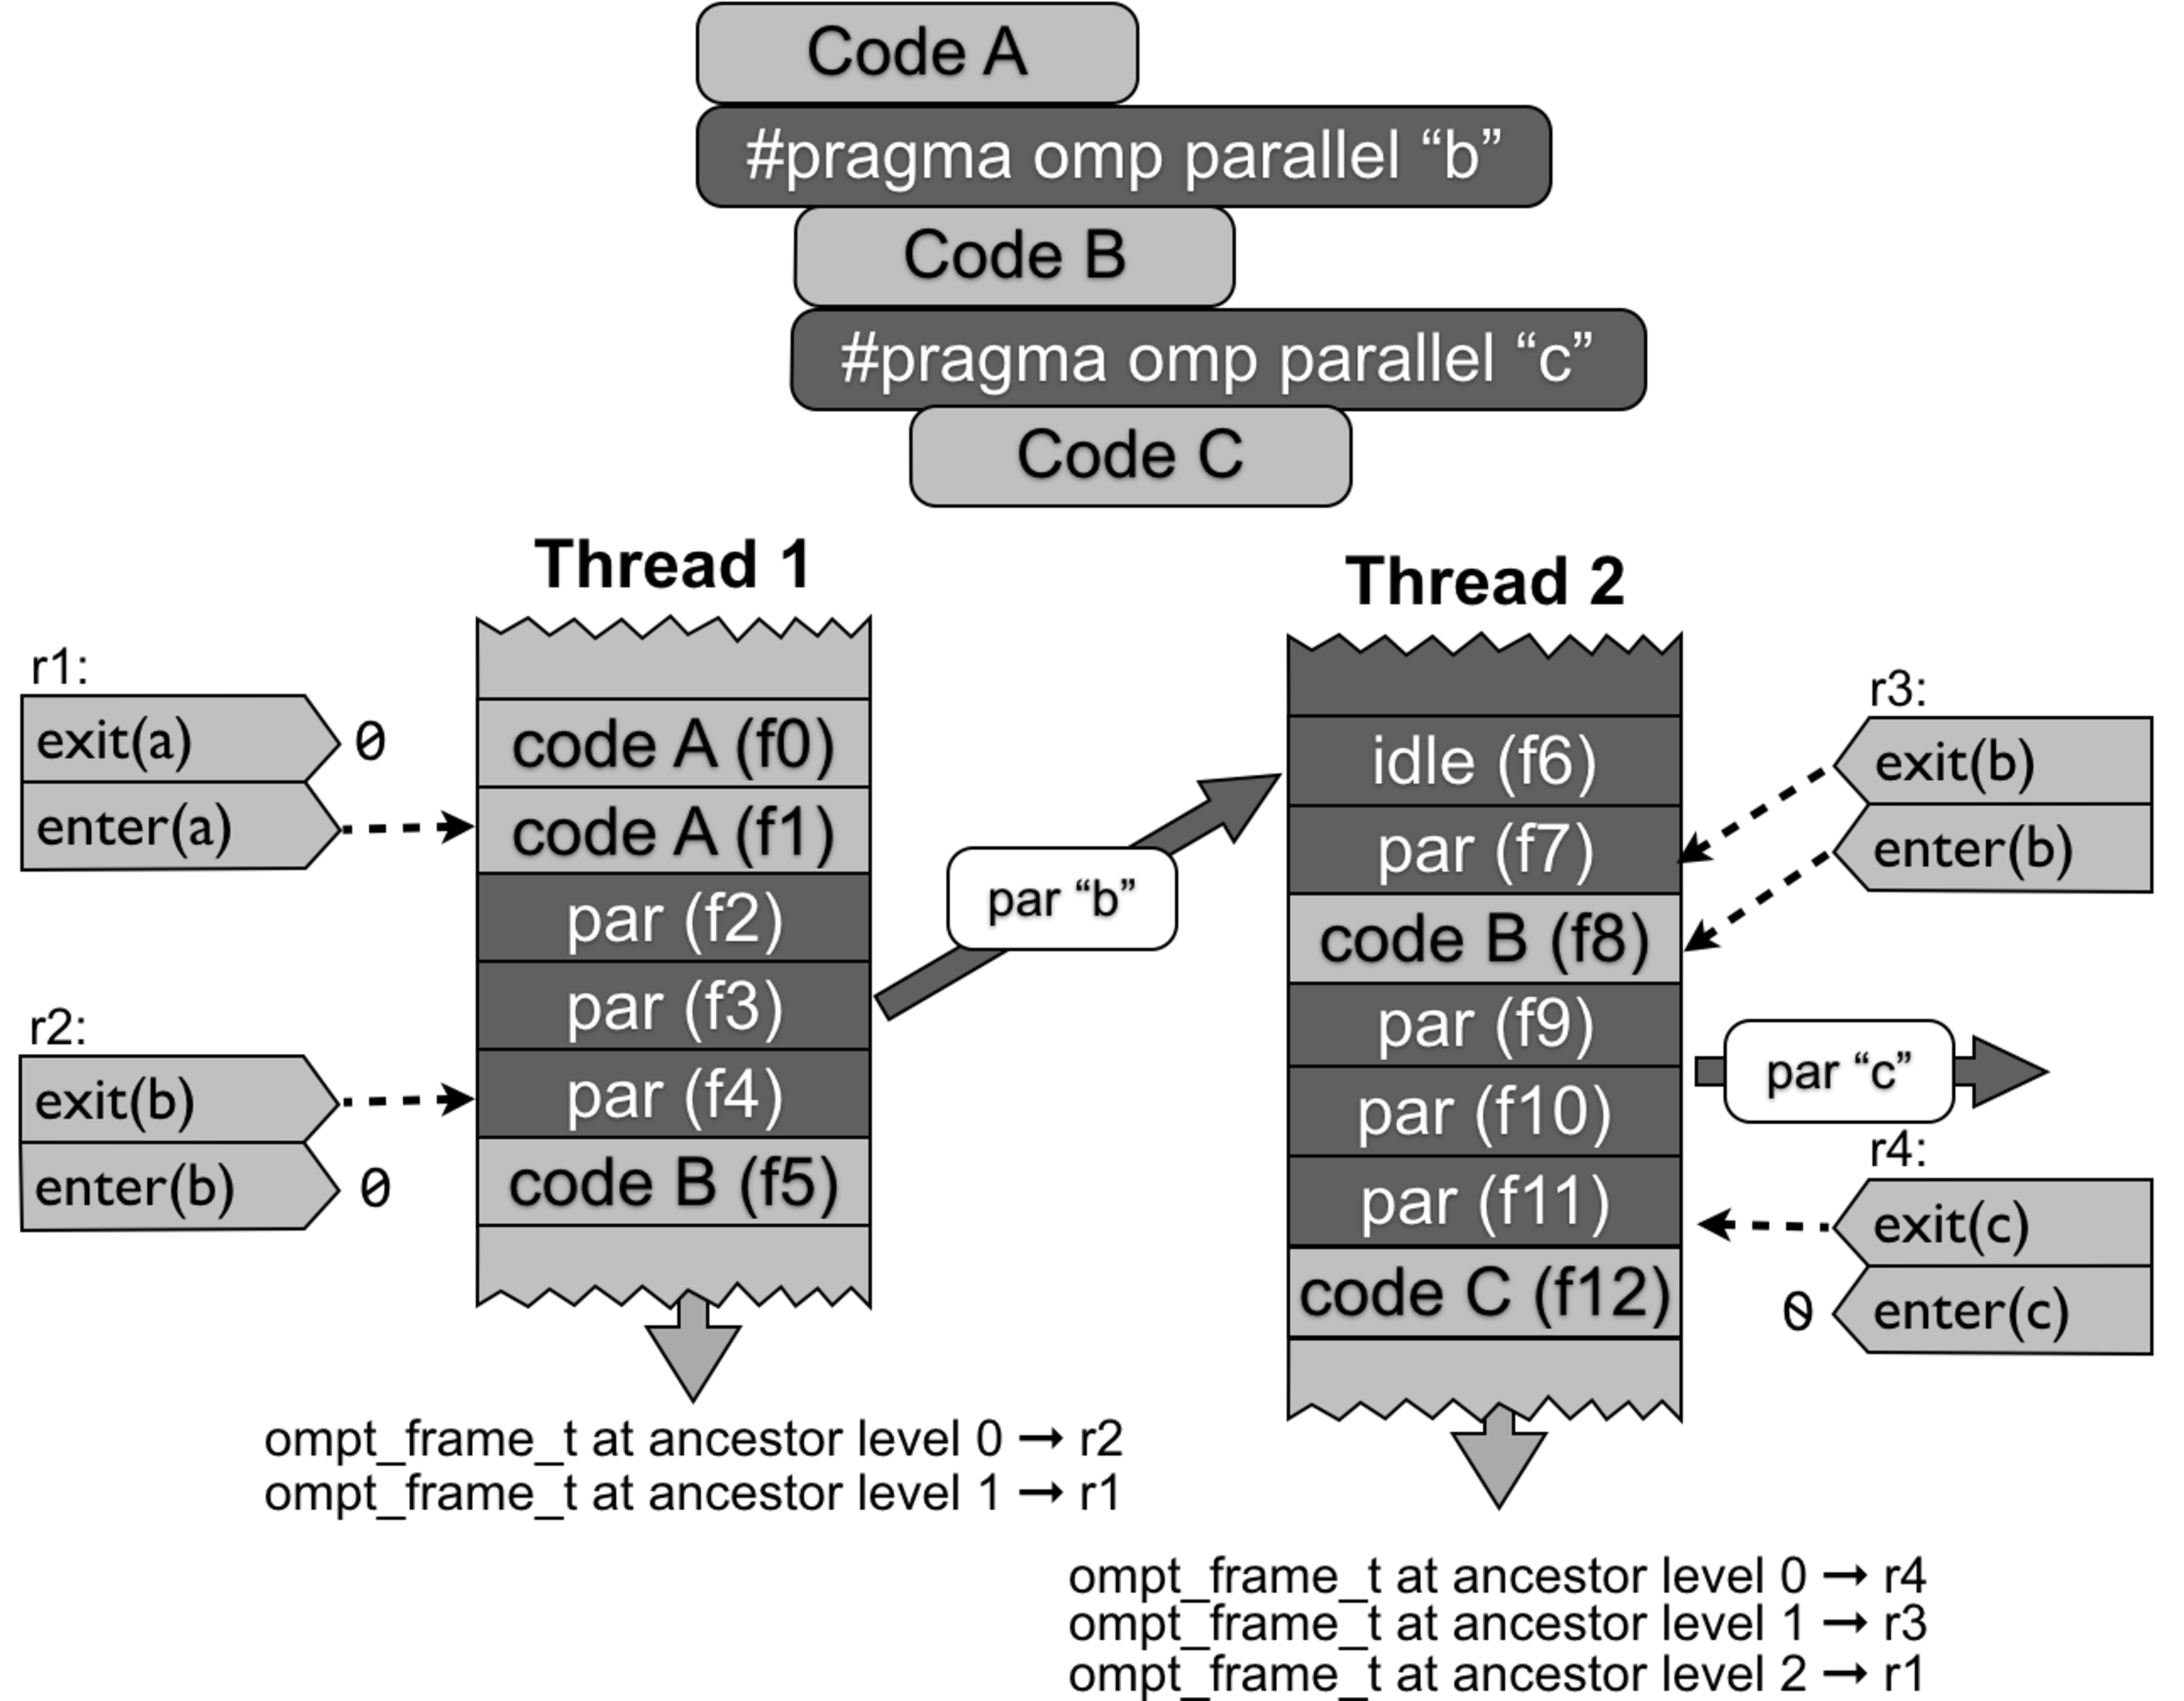
\includegraphics[scale=0.55]{callstack-cropped.pdf}
    \caption{Frame information.}
    \label{fig:frame}
\end{figure}

\sloppy
Figure~\ref{fig:frame} illustrates a program executing a nested parallel region, where code A, B, and C represent, respectively, code associated with an initial task, outer-parallel, and inner-parallel regions.  Figure~\ref{fig:frame}  also depicts the stacks of two threads, where each new function call instantiates a new stack frame below the previous frames. When thread 1 encounters the outer-parallel region (parallel ``b"), it calls a routine in the OpenMP runtime system to create a new parallel region. The OpenMP runtime sets the \verb|reenter_runtime_frame| field in the \verb|ompt_frame_t| for the initial task executing code A to  frame f2, the runtime routine called by frame f1 in the initial task. The  \verb|ompt_frame_t| for the initial task is labeled  \verb|r1| in Figure~\ref{fig:frame}. In this figure, three consecutive runtime system frames (labeled ``par'' with frame identifiers f2--f4) are on the stack. 
Before starting the implicit task for parallel region ``b" in thread 1, the runtime sets the \verb|exit_runtime_frame| in the implicit task's \verb|ompt_frame_t|  (labeled \verb|r2|) to f4. Execution of application code for parallel region ``b''  begins on thread 1  when the runtime system invokes application code B (frame f5) from frame f4. Since thread 1 is an OpenMP initial thread, a call to  \verb|ompt_get_idle_frame|  on this thread will always return NULL.

Let us focus now on thread 2, an OpenMP thread. Figure~\ref{fig:frame}  shows this worker executing  work for the outer-parallel region ``b."
On the OpenMP thread's stack is a runtime frame labeled ``idle,'' where the OpenMP thread waits for work. 
At any time after the idle frame is on thread 2's stack, a call to \verb|ompt_get_idle_frame| by thread 2 will return frame f6. 
When work becomes available, the runtime system invokes a function to dispatch it. While dispatching parallel work might involve a chain of several calls, here we assume that the length of this chain is 1 (frame f7).  Before thread 2 exits the runtime to execute an implicit task for parallel region ``b,'' the runtime 
sets the \verb|exit_runtime_frame| field of the implicit task's \verb|ompt_frame_t| (labeled \verb|r3|) to frame f7. 
When thread 2 later encounters the inner-parallel region ``c,"  execution returns to the runtime and the runtime fills in the  \verb|reenter_runtime_frame| field of the current task's \verb|ompt_frame_t| (labeled \verb|r3|) to frame f9. Before the task for parallel region ``c'' is invoked on thread 2, the runtime system sets the \verb|reenter_runtime_frame| field  of the \verb|ompt_frame_t| (labeled \verb|r4|) for the implicit task for ``c'' 
to frame f11. Execution of application code for parallel region ``c''  begins on thread 2  when the runtime system invokes application code C (frame f12) from frame f11.


Below the stack for each thread in Figure~\ref{fig:frame}  is set of \verb|ompt_get_task_frame| inquiries that are assumed to be made on each thread for the stack state shown. Each call indicates an ancestor level with an argument and shows the ID of the \verb|ompt_frame_t| record returned. Note that thread 2 has task frame information for three levels of tasks, whereas thread 1 has only two.


\end{document}
